\chapter{La Derivada}	\label{ch-la-derivada}

	\section{Intoducción histórica}
	
	En cálculo diferencial y análisis matemático, la derivada de una función es la razón de  cambio instantánea con la que varía el valor de dicha función matemática, según se  modifique el valor de su variable independiente. La derivada de una función es un \emph{concepto local}, es decir, se calcula como el límite de la rapidez de cambio media de la función en cierto intervalo, cuando el intervalo considerado para la variable independiente se torna cada vez más pequeño. Por eso se habla del valor de la derivada de una función en un punto dado.
		
	
	Un ejemplo habitual aparece al estudiar el movimiento: si una función representa la posición de un objeto con respecto al tiempo, su derivada es la velocidad de dicho objeto para todos los momentos. Un avión que realice un vuelo transatlántico de 
$4500 km$ entre las $12:00$ y las $18:00$, viaja a una velocidad media de $750 km/h$. Sin embargo, puede estar viajando a velocidades mayores o menores en distintos tramos de la ruta. En particular, si entre las $15:00$ y las $15:30$ recorre $400 km,$ su velocidad media en ese tramo es de $800 km/h$. Para conocer su velocidad instantánea a las $15:20$, por ejemplo, es necesario calcular la velocidad media en intervalos de tiempo cada vez menores alrededor de esta hora: entre las $15:15$ y las $15:25$, entre las $15:19$ y las $15:21$.
	
El valor de la derivada de una función en un punto también puede interpretarse geométricamente, ya que se corresponde con la pendiente de la recta tangente a la gráfica de la función en dicho punto. La recta tangente es, a su vez, la gráfica de la mejor aproximación lineal de la función alrededor de dicho punto. 

\underline{Historia de la derivada}.
	
Los problemas típicos que dieron origen al cálculo infinitesimal comenzaron a plantearse en la época clásica de la antigua Grecia (siglo III a. C.), pero no se encontraron métodos sistemáticos de resolución hasta diecinueve siglos después (en el siglo XVII por obra de Isaac Newton y Gottfried Leibniz).
	
	En lo que atañe a las derivadas existen dos conceptos de tipo geométrico que le dieron origen:
	

		\hspace{5mm} * El problema de la tangente a una curva (Apolonio de Perge)
		
		\hspace{5mm} * El Teorema de los extremos: máximos y mínimos (Pierre de Fermat)
	
	En su conjunto dieron origen a lo que actualmente se conoce como cálculo diferencial.
	
	
	En el siglo XVII, los matemáticos perdieron el miedo que los griegos les habían tenido a los infinitesimales: Johannes Kepler y Bonaventura Cavalieri fueron los primeros en usarlos, empezaron a andar un camino que llevaría en medio siglo al descubrimiento del cálculo infinitesimal.
	
	A mediados del siglo XVII las cantidades infinitesimales fueron cada vez más usadas para resolver problemas de cálculos de tangentes, áreas, volúmenes; los primeros darían origen al cálculo diferencial, los otros al cálculo integral.

	A finales del siglo XVII se sintetizaron en dos conceptos los algoritmos usados por sus predecesores, en lo que hoy llamamos `derivada' e `integral'. La historia de la matemática reconoce que Isaac Newton y Gottfried Leibniz son los creadores del cálculo diferencial e integral. Ellos desarrollaron reglas para manipular las derivadas (reglas de derivación) e Isaac Barrow demostró que la derivación y la integración son operaciones inversas.
	

	Newton desarrolló en Cambridge su propio método para el cálculo de tangentes. En 1665 encontró un algoritmo para derivar funciones algebraicas que coincidía con el descubierto por Fermat. A finales de 1665 se dedicó a reestructurar las bases de su cálculo, intentando desligarse de los infinitesimales, e introdujo el concepto de \emph{fluxión}, que para él era la velocidad con la que una variable `fluye' (varía) con el tiempo.

	Gottfried Leibniz, por su parte, formuló y desarrolló el cálculo diferencial en 1675. Fue el primero en publicar los mismos resultados que Isaac Newton descubriera 10 años antes, de manera independiente. En su investigación conservó un carácter geométrico y trató a la derivada como un \emph{cociente incremental} y no como una velocidad, viendo el sentido de su correspondencia con la pendiente de la recta tangente a la curva en dicho punto.
	
	Leibniz es el inventor de diversos símbolos matemáticos. A él se deben los nombres de cálculo diferencial y cálculo integral, así como los símbolos de derivada $\; \dfrac {dy}{dx}\; $ y del símbolo integral $\int$.

	
	\section{Concepto de derivada. Interpretación geométrica y física}
	\label{IG-derivada}
	
	
	La derivada de una función puede interpretarse geométricamente como la pendiente de una curva, y físicamente como una razón `instantánea' de cambio. 
	
	\subsection{Tangente a una curva}
	 
	En la primera mitad del siglo XVII no se conocían métodos generales para calcular la tangente a una curva en un punto de la misma. Este problema se presentaba con frecuencia en mecánica, en óptica y en geometría, y generalmente se resolvía, de forma geométrica, con técnicas adaptadas a cada caso particular. La dificultad está en que, siendo la tangente una recta, se precisa conocer dos puntos de la misma, o bien un punto y su pendiente, para poderla determinar. 
	 
	 Supongamos que queremos hallar la tangente a una curva de ecuación cartesiana $y = f (x)$ en el punto $(a, f (a))$. La estrategia, usada primero por Pierre de Fermat y más tarde por Newton, consiste en aproximar la tangente por rectas secantes cuyas pendientes sí pueden calcularse directamente. En particular, consideremos la recta que une el punto $(a, f (a))$ con un punto cercano, $(x, f (x))$, de la gráfica de $f$ . Esta recta se llama una secante (recta que corta a la curva, pero no es tangente a la curva). La pendiente de esta secante es: $\dfrac {f(x) -f(a)} {x-a}$ dicho número suele llamarse \emph{cociente incremental} de $f$ en $a$. 
	 
	 \begin{multicols}{2}
	 	
	 

     
	Observa que una secante es una buena aproximación de la tangente, siempre que el punto $(x, f (x))$ esté próximo a $(a, f (a))$. Estas consideraciones llevan a definir la tangente a la gráfica de $f$ en el punto $(a, f (a))$ como la recta que pasa por dicho punto y cuya pendiente es igual al límite: $\underset{x\to a}{lim}\;{\dfrac {f(x)-f(a)}{x-a}}$ supuesto, claro está, que dicho límite exista. 
	
	 \begin{figure}[H]
			\centering
			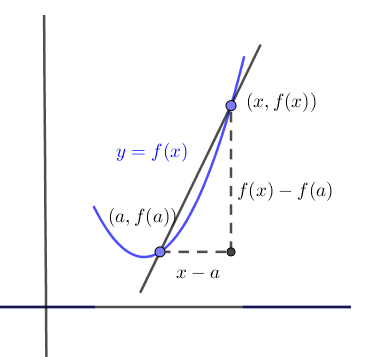
\includegraphics[width=0.4\textwidth]{imagenes/imagenes04/T04IM01.png}
			\caption {Recta secante.}
		\end{figure}
   
		\end{multicols}
		
\subsection{Razón de cambio puntual y velocidad instantánea}
	  
Muchas leyes de la Física, la Química, la Biología o la Economía, son funciones que relacionan una variable `dependiente' $y$ con otra variable `independiente' $x$, lo que suele escribirse en la forma $y = f(x)$. Si la variable independiente cambia de un valor inicial $a$ a otro $x$, la variable $y$ lo hace de $f(a)$ a $f(x)$. La razón de cambio promedio o \emph{`tasa de variación media'} de $y = f(x)$ con respecto a $x$ en el intervalo $[a, x]$ es: $\dfrac {f(x)-f(x)}{x-a}$
	  
	  Con frecuencia interesa considerar la razón de cambio en intervalos cada vez más pequeños. Esto lleva a definir lo que podemos llamar `razón de cambio instantáneo' o \emph{`tasa de variación instantánea'} de $y = f (x)$ con respecto a $x$ en el punto $a$ como: $\underset {x\to a}{lim}\;{\dfrac {f(x)-f(a)}{x-a}}$

	  El ejemplo más conocido de esto que decimos es el de un móvil que se mueve a lo largo de una recta sobre la cual hemos elegido un origen. Sea $s(t)$ la posición del móvil en el tiempo $t$, es decir, la distancia con signo del móvil al origen en el tiempo $t$. La razón de cambio promedio tiene en este caso una interpretación física natural: $\dfrac{s(a+h)-s(a)}{h}$ 
	  
	  Es la velocidad media del móvil en el intervalo de tiempo comprendido entre $a$ y $a + h$. Parece intuitivo que, en cada instante, el móvil se mueve con una determinada velocidad instantánea. Pero no hay manera de medir directamente una velocidad instantánea; un instante quiere decir una posición en la recta: la velocidad instantánea del móvil para $t = a$ es la velocidad que tiene cuando está en la posición $s(a)$. La velocidad instantánea es una abstracción de un característica física del movimiento, pero no es una magnitud que podamos observar directamente. La única definición razonable de velocidad instantánea es como la razón de cambio puntual (tasa de variación instantánea): $\underset{h\to 0}{lim}\:{\dfrac {s(a+h)-s(a)}{h}}$.
	  
	  \subsection{Definición de derivada}
	  
	  \begin{defi}
	  Se dice que $f:I\to \mathbb R$ es `devivable' en un punto $a\in I$, y se denota por $f'(a)$, si existe y es finito el límite:	
	  
	  \begin{equation}
	  	\boxed{	\quad f'(a)=\underset {x\to a}{lim}\;{\dfrac{f(x)-f(a)}{x-a}}\; \in \mathbb R \quad}
	  \end{equation}
	  
	  
	  Una notación totalmente equivalente se consigue al sustituir $x$ por $a+h$, si $x\to a$, entonces $a+h \to a$, o, lo que es lo mismo, $h\to 0$ y tenemos:
	  
	  \begin{equation}
	  		\boxed{\quad f'(a)=\underset {h\to 0}{lim}\;{\dfrac{f(a+h)-f(a)}{h}} \; \in \mathbb R \quad }
	  \end{equation}
	  
	  Esta \textbf{notación $f'(a)$} para la derivada de una función en un punto es debida a \textbf{Lagrange}. 
	  
	  Nótese que la derivada de una función en un punto es un número real.
	  \end{defi}
	  
	  $\divideontimes$ Atendiendo a la definición formal de límite vista en el capítulo anterior (definición \ref{defi:limite}), $f$ es `derivable' en $a$ si existe un número $f'(a)$ de modo que para cualquier $\varepsilon>0$, por pequeño que sea, somos capaces de encontrar un $\delta>0$ tal que para todo $x\in I, \; x\neq a$ y con $|x-a|<\delta$ se cumple que $\left|\dfrac {f(x)-f(a)}{x-a} - f'(a) \right|<\varepsilon$
	  
	  
	  \section{Función derivada}
	  
	  \begin{defi}
	  Sea $f:I\to \mathbb R$, derivable en todo punto de $I$. Llamamos función derivada de $f$ y la representamos por $f'$ a la función: $f':I\to \mathbb R$ tal que a cada punto $x\in I$ le hace corresponder su derivada en ese punto, $f'(x)$.	
	  \end{defi}
	  
	  \subsection{Otras notaciones para las derivadas}
	  
	   \begin{multicols}{2}
	   $\quad$
	   
	  Aparte de la \textbf{notación de Lagrange: $f'(x)$} que acabamos de ver, hay otras notaciones para las derivadas.
	  	\begin{figure}[H]
			\centering
			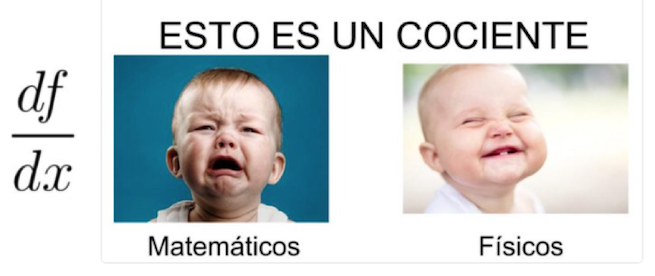
\includegraphics[width=0.5\textwidth]{imagenes/imagenes04/xiste04.png}
			\label{mates-fisics}
		\end{figure}
		\end{multicols}
	
	\vspace{-5mm}
	
	  Notación de \textbf{diferencial de Leibniz, $\dfrac {\dd f(x)}{\dd x} $}. Se lee derivada de $f(x)$ respecto de $x$. Esta notación tiene la ventaja de sugerir la derivada como cociente de elementos infinitesimales (diferenciales) y es muy usada en física. Veremos su enorme utilidad práctica y enorme sencillez cuando estudiemos la derivada de las funciones compuestas y la derivada de la función inversa.
	  
	
	  Con esta notación, la derivada de una función en un punto se representa como:  $\eval{ \dfrac {\dd f(x)}{\dd x} }_{x=a} $, o también como $\left( \dfrac {\dd f(x)}{\dd x}  \right)\; (a)$
	  
	  
	  
	  
	  Notación de \textbf{Newton: $ \dot { y }=y' $}. Esta notación, aunque incómoda, sigue utilizándose en mecánica para referirse a la derivada temporal de una variable:  $\dot {x}= \dfrac {\dd x(t)}{\dd t}=x'(t)$

	  
	Notación de \textbf{Euler: $D_x \; f=f'(x)$}
	
	\subsection{Rectas Tangente y Normal a una función en un punto. Elementos de una curva relacionados con la derivada}
	 \label{subsec:RTN} 
	  
	  \begin{defi}Recta tangente a una curva. Supuesto $f$ derivable en $a$, la ecuación:
	  
	  \begin{equation}
	  	\boxed{\; y-f(a)=f'(a)\cdot(x-a) \; }
	  	\label{eq:recta-tangente}
	  \end{equation}
	  	
	  	Es la ecuación de la recta tangente a $f(x)$ en el punto $(a,f(a))$
	  \end{defi}
	  
	  \begin{defi}Recta Normal a una curva. Supuesto $f$ derivable en $a$, con $f'(a)\neq 0$, la ecuación:
	  
	  \begin{equation}
	  	\boxed{ \; y-f(a)=-\dfrac 1 {f'(a)}\cdot(x-a) \; }
	  	\label{eq:recta-normal}
	  \end{equation}
	  	
	  	Es la ecuación de la recta normal (perpendicular) a $f(x)$ en el punto $(a,f(a))$
	  \end{defi}
	  
	  
	   $\divideontimes$ \textbf{Elementos de una curva relacionados con la derivada.}
	  
	 \begin{figure}[H]
		\centering
		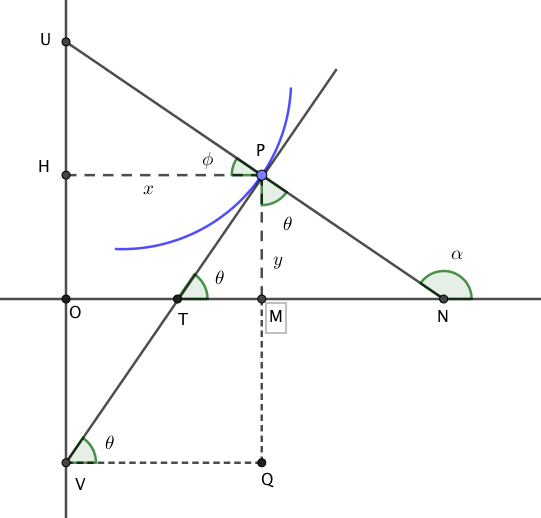
\includegraphics[width=0.5\textwidth]{imagenes/imagenes04/T04IM02.png}
		\caption {Elementos de una curva relacionados con la derivada.}
	\end{figure}
	
	\begin{itemize}
		\item La pendiente de la recta tangente (la que pasa por los puntos VP) es $\tan \theta = y'$.
		\item La pendiente de la recta normal (la que pasa por los puntos UN) es $\tan \alpha = \tan (\pi/2 + \alpha)=-1/y'$.
		\item El segmento $\overline {TM}$ es la \textbf{subtangente}. Su longitud viene dada por $\overline  {TM}=y \; \cot( \theta ) = y/y'$ 
		\item El segmento $\overline{MN}$ es la \textbf{subnormal}. Su longitud viene dada por $\overline{MN}=y\; \tan(\theta)=yy'$.	
		\item Los segmentos interceptados por los ejes $OX$ y $OY$ con la tangente son:
		
		
		\begin{equation*}
		\begin{cases}
		\overline{OT}=\overline{OM}-\overline{TM}=x-y/y'  \\ 
		\overline{OV}=\overline{PM}-\overline{PQ}=y-x\; \tan(\theta)=y-xy'   
		\end{cases}
		\end{equation*}
		
		
		\item Los segmentos interceptados por los ejes $OX$ y $OY$ con la normal son:
		
		\begin{equation*}
		\begin{cases}
			\overline{ON}=\overline{OM}+\overline{MN}=x+y\; \tan (\theta)=x+yy'  \\ 
			\overline{OU}
			=\overline{OH}+\overline{HU}=y+x\; \tan (\phi)=y+x\; \tan (\pi/2 - \theta)=y+x/y' 
		\end{cases}
		\end{equation*}
		
	%\begin{equation*}
	%\begin{pmatrix*}[l]
	%\overline{OT}=\overline{OM}-\overline{TM}=x-y/y'  \\ 
	%\overline{OV}=\overline{PM}-\overline{PQ}=y-x\; \tan(\theta)=y-xy' 
	%\end{pmatrix*}
	%\end{equation*}
		
		
		\end{itemize}
	
	
	 \begin{figure}[H]
			\centering
			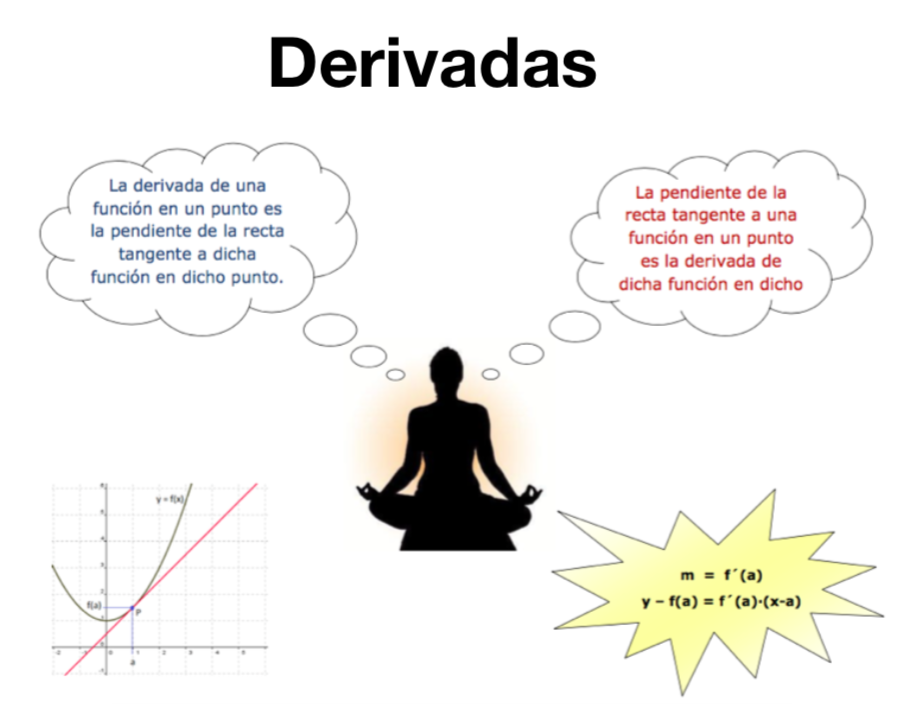
\includegraphics[width=0.9\textwidth]{imagenes/imagenes04/T04IM07.png}
			\caption {Recuerda la interpretación de derivada.}
			\label{img:mantra-derivada}
	\end{figure}
	
	
	
	\section{Derivadas laterales}
	
	\begin{defi} Derivadas laterales.
	
	Decimos que \textbf{$f$ es derivable por la izquierda en $a$}, y lo representamos por $f'_{-}(a)$ (análogamente \textbf{ $f$derivable por la derecha en $a$}, $f'_{+}(a)$) si existen y son finitos los límites:
	
		\begin{equation}
		\label{ref:derivada-lateral}
			f'_{-}(a)=\underset{x\to a^-}{lim}\;{\dfrac {f(x)-f(a)}{x-a}} \qquad ; \qquad f'_{+}(a)=\underset{x\to a^+}{lim}\;{\dfrac {f(x)-f(a)}{x-a}}
		\end{equation}
		
		Analogamente:
		\begin{equation}
			f'_{-}(a)=\underset{h\to 0^-}{lim}\;{\dfrac {f(a+h)-f(a)}{h}} \qquad ; \qquad f'_{+}(a)=\underset{h\to 0^+}{lim}\;{\dfrac {f(a+h)-f(a)}{h}}
		\end{equation}
		
		
		Teniendo en cuenta la relación entre límites y límites laterales, está claro que una función es derivable en un punto si existen, son finitas y coinciden sus derivadas laterales.
		
		\begin{equation}
			\exists f'(a) \leftrightarrow \exists f'_-(a), \; \exists f'_+(a) \; \wedge \; f'_-(a)=f`_+(a)
		\end{equation}
		
	\end{defi}
	
	\begin{multicols}{2}
		
	Cuando en una función $f$ continua en un punto $a$ las derivadas laterales existen, son finitas, pero distintas, decimos que en $a$ la función tiene un 	\emph{Punto Anguloso}, hay no una sino dos rectas tangentes distintas a la izquierda y a la derecha de $a$. Así como intuitivamente una función es continua en un punto si se puede dibujar, en un entorno de ese punto, sin `levantar el lápiz del papel', una función será derivable si \underline{además} el comportamiento en un entorno de ese punto es \emph{suave}, no abrupto, como aparece el la imagen de al lado.
	
	\begin{figure}[H]
		\centering
		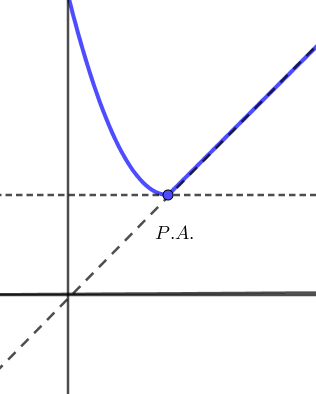
\includegraphics[width=0.3\textwidth]{imagenes/imagenes04/T04IM03.png}
		\caption {Punto anguloso.}
	\end{figure}
	
	\end{multicols}
	
	
	\section{Relación entre continuidad y derivabilidad}
	
	
	El siguiente teorema demuestra que la condición de derivabilidad es más fuerte o restrictiva que la de continuidad.
	
	\begin{teor}
	\label{teor:deriv-cont}
		Todo función derivable en un punto, es continua en él.
	\end{teor}

	\begin{proof}
		Sea $f:I\to \mathbb R$, derivable en $a$, es decir, $\exists f'(a)=\underset{x\to a}{lim}\;{\dfrac {f(x)-f(a)}{x-a}} \in \mathbb R$
		
		Consideremos la igualdad: $f(x)=f(a)+(x-a) \cdot \dfrac {f(x)-f(a)}{x-a} \qquad x\in I; \; x\neq a $, tomando límites cuando $x\to a$ se deduce que:
		
		$\underset {x\to a}{lim }{f(x)}= \underset {x\to a}{lim }{ f(a)+{(x-a)} \cdot \dfrac {f(x)-f(a)}{(x-a)} }=f(a)+\cancelto {0}{(x-a)} \cdot f'(a)= f(a)$, lo que indica que f(x) es continua en $a$.
		
	\end{proof}
	
	Obviamente, si una función no es continua en en punto no se podrá trazar una recta tangente en él, por lo que será no-derivable. Pero el hecho de que sea continua no asegura que sea derivable.
	
	El recíproco del teorema anterior no se cumple, no todas las funciones continuas son derivables, sirva como contraejemplo la figura anterior o, incluso, la función valor absoluto.
	
	
		\begin{figure}[H]
			\centering
			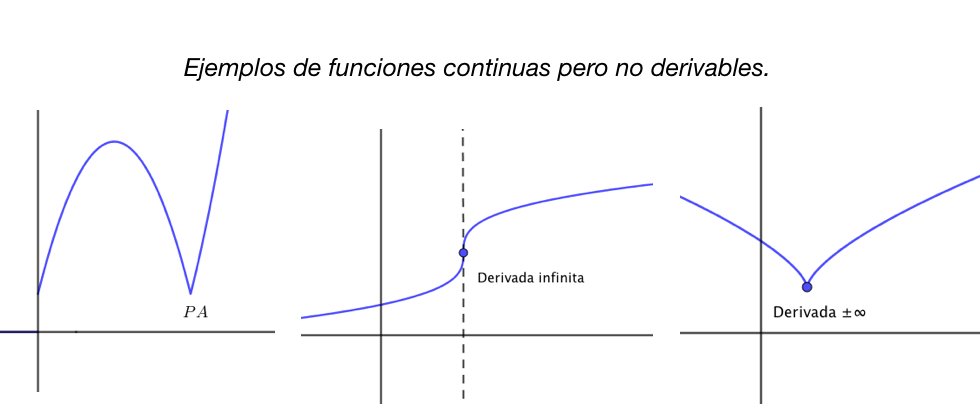
\includegraphics[width=0.8\textwidth]{imagenes/imagenes04/T04IM06.png}
			\caption{Funciones continuas y no derivables.}
		\end{figure}
		
		\begin{figure}[H]
			\centering
			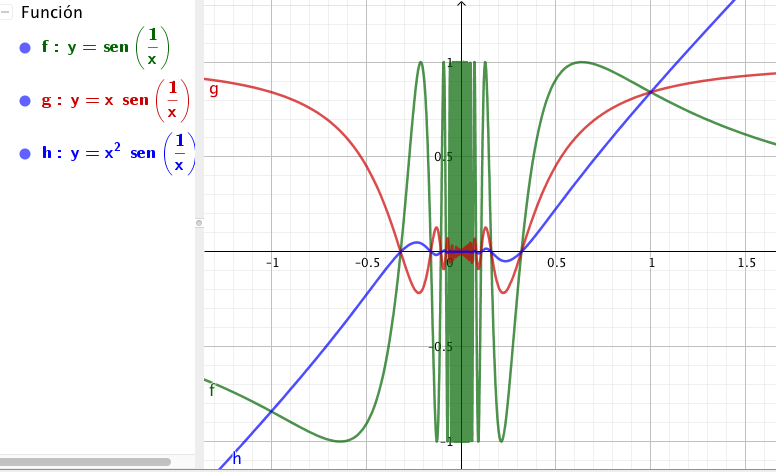
\includegraphics[width=0.6\textwidth]{imagenes/imagenes04/T04IM08.png}
			\caption{Verde: no continua en cero; Roja: continua en cero, pero no derivable; azul: continua y derivable en cero.}
			\label{fig:ctndaddvbdad}
		\end{figure}
		
		
	
	\begin{ejem} Calcular la derivada de la función $f(x)=|x|$ en el punto $a=0$
		
	\begin{multicols}{2}
		

	$f'(0)=\underset{h\to 0}{lim}\;{\dfrac {f(0+h)-f(0)} {h}}=\underset {h\to 0}{lim}\; {\dfrac {f(h)}{h}}$. Es necesario estudiar límites laterales (derivadas laterales) pues $0$ es el nexo de la función a trozos valor absoluto de $x$.
	
	$f'_-(0)=\underset{h\to 0^-}{lim}\;{\dfrac {-h}{h}}=-1 \qquad f'_+(0)=\underset{h\to 0^+}{lim}\;{\dfrac {+h}{h}}=+1$
	
	Como $f'_-(0)=-1\neq 1=f'_+(0) \to \nexists f'(0)$, la función no es derivable en el $0$, aunque sí continua, por lo que en $0$ la función presenta un punto anguloso.
	
	\begin{figure}[H]
			\centering
			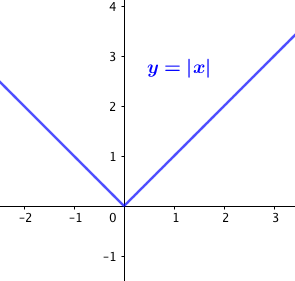
\includegraphics[width=0.4\textwidth]{imagenes/imagenes04/T04IM04.png}
			\caption{Función Valor Absoluto.}
		\end{figure}
		
	\end{multicols}
	
	\end{ejem}
	
	\begin{ejem} Usando la definición de derivada, calcula las rectas tangente y normal a $f(x)=2x^2+3x+1$ en el punto $a=-1 \qquad $\scriptsize{\textcolor{gris}{$f'(x)=4x+3 \to f'(-1)=4(-1)+3=-1$}}
	
	\normalsize
	Usemos una de las dos definiciones:
	
	$f('-1)=\underset {x\to -1}{lim}\;{\dfrac {f(x)-f(-1)}{x-(-1)}}= \underset {x\to -1}{lim}\;{\dfrac {2x^2+3x+1-0}{x+1}}=\underset {x\to -1}{lim}\;{\dfrac {2x^2+3x+1}{x+1}}=[0/0; \; ind]= \underset {x\to -1}{lim}\;{\dfrac {\cancel{(x+1)}(2x+1)}{\cancel{(x+1)}}}=\underset {x\to -1}{lim}\;{(2x+1)=2(-1)+1=-1}$
	
	Usando la otra definición:
	
	$f'(-1)=\underset {h\to 0}{lim}\; {\dfrac {f(-1+h)-f(-1)} {h}}= \underset {h\to 0}{lim}\; {\dfrac {2(-1+h)^2+3(-1+h)+1-0} {h}}=$
	
	$=\underset {h\to 0}{lim}\; {\dfrac {2(-1+h)^2+3(-1+h)+1-0} {h}}= \underset {h\to 0}{lim}\; {\dfrac {2h^2-h} {h}}=[0/0;\; ind]=$
	
	$ = \underset {h\to 0}{lim}\; {\dfrac {\cancel{h}(2h-1} {\cancel{h}}}=\underset {h\to 0}{lim}\; {(2 \cancelto{0}{h} - 1)}=-1$
	
	En cada caso, una de las dos definiciones es más útil que la otra.
	
	Puesto que tanto la recta tangente como la normal pasan por el punto $(-1,f(-1))=(-1,0)$ y teniendo en cuenta las ecuaciones de ambas rectas, ecuación \ref{eq:recta-tangente} y ecuación \ref{eq:recta-normal}, tenemos:
	
	Recta tangente a $f(x)$ en $x=-1 \quad \to \quad y-0=-1(x-(-1)); \quad y=-x-1$
	
	Recta normal a $f(x)$ en $x=-1 \quad \to \quad y-0=-\dfrac {1}{-1}(x-(-1)); \quad y=x+1$
	
	\end{ejem}
	
	\begin{ejem}  $\divideontimes$
	
	Dada la función $f(x)=\frac 1 2 x^2-2x+3$, calcula	$f'(4)$, las rectas tangente y normal en $x=4$ y los segmentos subtangente y subnormal.
	
	Es fácil comprobar que $f'(4)=2$, que la recta tangente es $y=2x-5$ y la recta normal $y=-\frac 1 2 x +5$. El segmento subtangente mide $6$ y el subnormal $1.5$
	
		\begin{figure}[H]
			\centering
			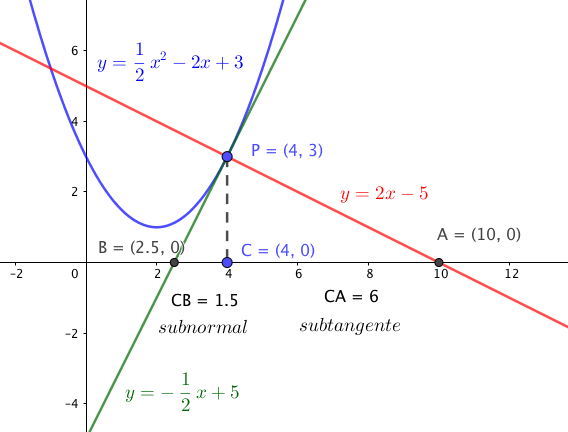
\includegraphics[width=0.7\textwidth]{imagenes/imagenes04/T04IM05.png}
			\caption{Subtangente y subnormal.}
		\end{figure}
	
	\end{ejem}
	
	\begin{ejem} Aplicando la definición de derivada, calcula $f'(2)$ a la función: $f(x)=\dfrac {2x}{x-1}$.
	
	$f'(2)=\underset {h\to 0}{lim}\;{\dfrac {f(2+h)-f(2)}{h}}= \underset {h\to 0}{lim}\;{\dfrac { \dfrac{2(2+h)}{(2+h)-1}-4}{h}} = \underset {h\to 0}{lim}\;{\dfrac {\dfrac {4+2h}{h+1}-4}{h}}=\underset {h\to 0}{lim}\;{\dfrac {4+2h-4(h+1)}{h(h+1)}}=\underset {h\to 0}{lim}\;{\dfrac {-2 \cancel{h}}{\cancel{h}(h+1)}}=\dfrac {-2}{1}=-2$
		
	\end{ejem}
	
	\begin{ejem} Calcula, aplicando la definición de derivada, $f'(4)$ para $f(x)=\sqrt{2x+1}$
	
	$f'(4)=\underset {x \to 4}{lim}\; {\dfrac {f(x)-f(4)}{x-4}}= \underset {x \to 4}{lim}\; {\dfrac {\sqrt{2x+1}-3}{x-4}}=[0/0\; ind]= \underset {x \to 4}{lim}\; {\left( \dfrac {\sqrt{2x+1}-3}{x-4}\cdot \dfrac {\sqrt{2x+1}+3}{\sqrt{2x+1}+3} \right) } = \underset {x \to 4}{lim}\; {\dfrac {2x+1-9}{(x-4)\cdot(\sqrt{2x+1}+3) }} = \underset {x \to 4}{lim}\; {\dfrac {2\cancel{(x-4)}}{\cancel{(x-4)}\cdot(\sqrt{2x+1}+3) }}= \underset {x \to 4}{lim}\; {\dfrac {2}{\sqrt{2x+1}+3 }}=\dfrac {2}{3+3}=\dfrac 2 6 =\dfrac 1 3$
		
	\end{ejem}
	
	\begin{ejem} Para la siguiente función, comprueba que en $x=1$ es continua, pero no derivable.
	
	\begin{equation*}
		f(x)=
		\begin{cases} 
		\;\;  3x-2 &\mbox{ si } x\le 1 \\ 
		\; x^2 & \mbox{ si } x>1 
		\end{cases}
	\end{equation*}
	
	Continuidad en x=1 (método de los tres pasos):
	
	$1) \quad \exists f(1)=3(1)-2=1$
	
	$2) \quad \exists \underset{x\to 1^-}{lim}\;{3x-2}=1=\underset{x\to 1^+}{lim}\;{x^2}=\underset{x\to 1}{lim}\;{f(x)}$
	
	$3) \quad $ Coinciden. Luego $f(x)$ continua en $x=1$
	
	Estudiemos ahora la derivabilidad en $x=1$:
	
	$1) \quad \exists f'_-(1)=\underset {x\to 1^-}{lim}\;{\dfrac {f(x)-f(1)}{x-1}}=\underset {x\to 1^-}{lim}\;{\dfrac {3x-2-1}{x-1}}=\underset {x\to 1^-}{lim}\;{\dfrac {3\cancel{(x-1)}}{\cancel{(x-1)}}}=3$
	
	$2) \quad \exists f'_+(1)=\underset {x\to 1^+}{lim}\;{\dfrac {f(x)-f(1)}{x-1}}= \underset {x\to 1^+}{lim}\;{\dfrac {x^2-1}{x-1}}=\underset {x\to 1^+}{lim}\;{\dfrac {(x+1)\cancel{(x-1)}}{\cancel{(x-1)}}}=2$
	
	$3) \quad f'_-(1)=3\neq 2=f'_+(1) \to \nexists f'(1)$ y la función es no derivable en $x=1$
	
	Tenemos una función que en $x=1$ es continua pero no derivable porque las derivadas laterales existen ambas, son finitas, pero distintas. Decimos que en $x=1$ la función $f(x)$ tiene un \emph{punto anguloso.}
	\end{ejem}
	
	\section{Álgebra de derivadas}
	
	\begin{teor}Álgebra de derivadas
	\label{teor:algebra-derivadas}
	
	Sean $f$ y $g$ dos funciones derivables en un cierto intervalo $I$ y sea $x\in I$, sea $k\in \mathbb R$, entonces se cumplen las siguientes reglas de derivación:
	
	\begin{itemize}
		\item $(k\cdot f)'(x)=k\cdot f'(x)$
		
		Derivada de constante por función: la constante no se deriva y se multiplica por la derivada de la función.
		
		\item $(f+g)'(x)=f'(x)+g'(x)$
		
		Derivada de la suma es igual a la suma de derivadas.
		
		\item $(f-g)'(x)=f'(x)-g'(x)$
		
		Derivada de la resta es igual a la resta de derivadas.
		
		\item $(f\cdot g)'(x)=f'(x)\cdot g(x)+f(x)\cdot g'(x)$
		
		Derivada del producto es igual a la derivada de la primera función por la segunda sin derivar, más la primera sin derivar por la derivada de la segunda función.
		
		\item $\left( \dfrac f g \right)'(x)=\dfrac {f'(x)\cdot g(x) - f(x)\cdot g'(x)}{g^2(x)}$
		
		Derivada del cociente es igual a la derivada del numerador por el denominador sin derivar, \underline{menos} el numerador sin derivar por la derivada del denominador; todo ello dividido por el denominador al cuadrado.

	\end{itemize}
	
			
	\end{teor}
	
	\begin{proof}
		
		$\divideontimes$  Demostraremos alguna de ellas:
		
		Derivada de la suma:
		
		$(f+g)'(x)=\underset {h\to 0}{lim}\;{\dfrac {(f+g)(x+h)-(f+g)(x)}{h}}=\underset {h\to 0}{lim}\;{\dfrac {f(x+h)+g(x+h)-(f(x)+g(x))}{h}}=\underset {h\to 0}{lim}\;{\left\{\dfrac {f(x+h)-f(x)}{h}+\dfrac {g(x+h)-g(x)}{h}\right\}}=\underset {h\to 0}{lim}\;{\dfrac {f(x+h)-f(x)}{h}}+ \underset {h\to 0}{lim}\;{\dfrac {g(x+h)-g(x)}{h}}=f'(x)+g'(x)$
		
		Derivada del cociente:
		
		$\left( \dfrac f g \right)'(x)=\underset{h\to 0}{lim}\;
		{ \dfrac { \left(\dfrac{f}{g}\right)(x+h)-\left(\dfrac{f}{g}\right)(x)   }{h}}= \underset {h\to 0}{lim}\;{\dfrac { \dfrac {f(x+h)}{g(x+h)} - \dfrac{f(x)}{g(x)} }{h}}=$
		
		$ =\underset {h\to 0}{lim}\; {\dfrac {f(x+h)g(x)-f(x)g(x+h) }{h g(x+h)g(x)}}= \underset {h\to 0}{lim}\; {\dfrac {f(x+h)g(x) \textbf{-f(x)g(x)+f(x)g(x)}-f(x)g(x+h) }{h \; g(x+h)\; g(x)}}=$
		
		$=\underset {h\to 0}{lim};{\dfrac {1}{g(x+h)g(x)} \cdot \left[ \dfrac {f(x+h)-f(x)}{h}\cdot g(x) - f(x)\cdot \dfrac {g(x+h)-g(x)}{h} \right]}=$
		
		$=\dfrac {1}{g^2(x)}[f'(x)g(x)-f(x)g'(x)]$
		
		
	\end{proof}
	
	\section{Derivadas de las funciones elementales}
	
	Demostraremos solo algunas de ellas.
	
	\begin{teor} Derivadas funciones elementales.
		
		\begin{itemize}
			\item $f(x)=k \to f'(x)=0$
			\item $f(x)=x \to f'(x)=1$
			\item $f(x)=x^n \to f'(x)=n\cdot x^{n-1}$
			\item $f(x)=a^x \to f'(x)=\ln a \cdot a^x; \quad f(x)=e^x \to f'(x)=e^x$
			\item $f(x)=\log_a x \to f'(x)=\dfrac {1}{\ln a \cdot x}; \quad f(x)=\ln x \to f'(x)=\dfrac 1 x$
			\item $f(x)=\sin x \to f'(x)=\cos x$
			\item $f(x)=\cos x \to f'(x)=-\sin x$
			\item $f(x)=\tan x =\dfrac {\sin x}{\cos x}\to f'(x)=1+\tan^2 x= \dfrac {1}{\cos^2 x}$
			\item etc. Ya ampliaremos todo esto en una tabla de derivadas.
		\end{itemize}
		
	\end{teor}

	\begin{proof}   $\divideontimes$ Demostraremos solo algunas de ellas.
	
	Derivada de la función identidad:
	
	$f(x)=x \to f'(x)=\underset{h\to 0}{lim}\;{\dfrac {f(x+h)-f(x)}{h}}=\underset {h \to 0}{lim}\;{\dfrac {x+h-x}{h}}=\underset{h\to 0}{lim}\;{1}=1$
	
	\vspace{4mm}Derivada de la función potencial:
	
	$f(x)=x^n \to f'(x)=\underset {h\to 0}{lim}\;{\dfrac {f(x+h)-f(x)}{h}}=\underset{h\to 0}{lim}\;{\dfrac {(x+h)^n - x^n}{h}}=$
	
	Teniendo en cuenta la fórmula del binomio de Newton demostrada en el ejercicio resuelto \ref{ejre:binomio-newton}:
	
	$= \underset {h\to 0}{lim}\;{\dfrac { \cancel{\left( \begin{matrix} n \\ 0 \end{matrix} \right) x^n} + \left( \begin{matrix} n \\ 1 \end{matrix} \right) x^{n-1}\; h + \left( \begin{matrix} n \\ 2 \end{matrix} \right) x^{n-2} h^2 + ... + \left( \begin{matrix} n \\ n-1 \end{matrix} \right) x h^{n-1} + \left( \begin{matrix} n \\ n \end{matrix} \right) h^n \; -\; \cancel{x^n}   }{h}}=$
	
	$=\underset{h\to 0}{lim}\;{\dfrac {\cancel{h}\cdot \left[\left( \begin{matrix} n \\ 1 \end{matrix} \right) x^{n-1)} + \left( \begin{matrix} n \\ 2 \end{matrix} \right) x^{n-2} \cancelto{0}{h} + \left( \begin{matrix} n \\ 3 \end{matrix} \right) x^{n-3}\cancelto{0}{h^2} + ... + \left( \begin{matrix} n \\ n \end{matrix} \right) \cancelto{0}{h^{n-1}}   \right]}{\cancel{h}}} =$
	
	$ = \left( \begin{matrix} n \\ 1 \end{matrix} \right) x^{n-1}= \dfrac {n!}{1!\cdot (n-1)!}x^{n-1}=n\; x^{n-1}$
	
	\vspace{4mm}Derivada de la función seno:
	
	$f(x)=\sin x \to f'(x)=\underset{h\to 0}{lim}\;{\dfrac {\sin(x+h)-\sin x}{h}}=  \underset{h\to 0}{lim}\;{\dfrac {(\cancel{\sin x} \; \cancelto{1}{\cos h} \; + \; \cos x\; \sin h)-\cancel{\sin x}}{h}}=$

	Teniendo en cuenta que $\underset {h\to 0}{lim}{\dfrac {\sin h}{h}}=1$ tal y como vimos en el ejemplo \ref{ejem:sinx/x}, tenemos que:	
	
	$=\underset{h\to 0}{lim}\;{\cos x \; \cancelto{1}{ \dfrac {\sin h}{h}} }=\cos x$
		
	\end{proof}
	
	
		\section{Ejercicios elementales de derivadas}
	
	Aunque estos ejercicios ya deben saberse del curso anterior, haremos y propondremos algunos como repaso.
	
	\subsection{Ejercicios resueltos de derivadas simples}
	
	
	\begin{ejre} Deriva las siguientes funciones:
	
	\begin{multicols}{2}
	
	\begin{enumerate}
		\item $f(x)=\sqrt x$
		\item $f(x)=\dfrac 1 x$
		\item $f(x)=\cot x$
		\item $f(x)=7x^3-4x^2-3x+5$
		\item $f(x)=\dfrac {3x-1}{5x^2-4}$
		\item $f(x)=e^x\cdot \sin x$
		\item $f(x)=\sqrt{x}\; e^x\; \cos x$
		\item $f(x)=\dfrac {\sin x + \cos x}{\sin x - \cos x}$
	\end{enumerate}
		
	\end{multicols}

		
	\end{ejre}
	
	
	
	\begin{proofw}\renewcommand{\qedsymbol}{$\diamond$}
	
	Resolvamos:
		
		\begin{enumerate}
			\item $y=\sqrt{x}=x^{\frac 1 2} \to y'=\frac 1 2 x^{\frac 1 2 - 1}= \frac 1 2 x^{-\frac 1 2}= \dfrac {1}{2 \sqrt {x}}$. 
			
			Como la raíz cuadrada es tan común en ciencia, vale la pena recordar su derivada. $y=\sqrt{x} \to y'=\dfrac {1}{2 \sqrt {x}}$
			\item $y=\dfrac 1 x = x^{-1}\to y'=-1\; x^{-1-1}=-1 x^{-2}=-\dfrac 1 {x^2}$
			
			Como en el caso anterior, al ser la inversa muy común también es conveniente recordar su derivada: $y=\dfrac 1 x \to y'=-\dfrac 1 {x^2}$
			
			\item $y=\cot x=\dfrac {\cos x}{\sin x} \to y'=\dfrac {(\cos x)'\cdot (\sin x) - (\cos x)\cdot (\sin x)' }{\sin^2 x}=\dfrac {-\sin^2 x - \cos^2 x}{\sin^2 x}= \dfrac {-1}{\sin^2 x}$
			
			\item $y=7x^3-4x^2-3x+5 \to y'=21x^2-8x-3$
			
			\item $y=\dfrac {3x-1}{5x^2-4} \to y'=\dfrac {3(5x^2-4)-(3x-1)10x}{(5x^2-4)^2}=\dfrac {-15x^2+10x-12}{(5x^2-4)^2}$
			
			\item $y=e^x \; \sin x \to y'= e^x \; \sin x +e^x \; \cos x=e^x\; (\sin x + \cos x) $
			
			\item $y=\sqrt{x} \; e^x \cos x = \sqrt{x} \; (e^x \cos x) \to y'= \dfrac {1}{2 \sqrt{x}}\cdot (e^x \cos x) + \sqrt{x} \cdot (e^x \cos x)' = \dfrac {1}{2 \sqrt{x}}\cdot (e^x \cos x) + \sqrt{x} \cdot (e^x \cos x + e^x (-\sin x)) = \dfrac {1}{2 \sqrt{x}}\cdot (e^x \cos x) + \sqrt{x} \cdot (e^x \cos x - e^x \sin x)$
			
			\item $y=\dfrac {\sin x + \cos x}{\sin x - \cos x} \to y'=\dfrac {(\cos x - \sin x)(\sin x - \cos x)-(\sin x + \cos x)(\cos x + \sin x)}{(\sin x - \cos x)^2}=\dfrac {-2}{(\sin x - \cos x)^2}$
			
		\end{enumerate}
		
	\end{proofw}

	
	
	\subsection{Ejercicios propuestos de derivadas simples}
	
	\begin{enumerate}
		\item $y=-\dfrac {x^3+x-1}{2} \qquad $ \textcolor{gris}{$\to \quad y'=-\frac 3 2 x^2-\frac 1 2$}
		\item $y=- \frac 2 {x^3}+ \frac 3 {x^2}-4x \qquad$ \textcolor{gris}{$\to \quad y'=\frac 6 {x^4}-\frac 6 {x^3}-4$}
		\item $y=\dfrac {5x^4-3x^3}{x^5} \qquad$ \textcolor{gris}{$\to \quad y'=-\frac 5 {x^2}+\frac 6 {x^3}$}
		\item $y=\sqrt{x^3} \qquad$ \textcolor{gris}{$\to \quad y'=\frac 3 2 \sqrt{x}$}
		\item $y=-3 \sqrt{x}-2 \sqrt[3]{x^2} \qquad$ \textcolor{gris}{$\to \quad y'= \dfrac{-3}{2\sqrt{x}}-\dfrac{4}{3\sqrt[3]{x}}$}
		\item $y=\dfrac{\sqrt{x}\; \sqrt[3]{x}}{\sqrt[4]{x}} \qquad $ \textcolor{gris}{$\to \quad y'=\dfrac {7}{12\; \sqrt[12]{x^5}}$}
		\item $y=\dfrac{e^x \; \sin x}{x^2 \; \ln x} \qquad$ \textcolor{gris}{$\to \quad y'= \dfrac {x^2 \ln x \; e^x (\sin x +\cos x)- e^x \sin x (2x \ln x + x)}{x^4 \ln^2 x}$ }
		
	\end{enumerate}
	
	\section{Derivada de la función compuesta: `Regla de la cadena'}
	
		\begin{teor} Regla de la Cadena.
	\label{teor:regla-cadena}	
	
	Sea $f:]a,b[\to \mathbb R$ y $g:]c,d[\to \mathbb R$ , con $Rec(f) \subset ]c,d[ \quad \to \quad (g\circ f)(x)=g(f(x))$
	
	Conocidos $f'(x)$ y $g'(x)$, se trata de encontrar $(g\circ f)'(x)$.
	
	Esta relación se conoce como la `derivada de la función compuesta' o `regla de la cadena' y es de enorme utilidad en el cálculo de derivadas.
	
	Demostraremos que, en las condiciones anteriores, se cumple que:
	
	\begin{equation}
		(g\circ f)'(x)=g'\left( f(x)\right) \cdot f'(x)
	\end{equation}
	
	\end{teor}
	
	\begin{proof}Calculemos $(g\circ f)'(x)$ aplicando la definición de derivada:
	
	$(g\circ f)'(x)=\underset {h \to 0}{lim}\; {\dfrac {(g \circ f)(x+h)-(g\circ f)(x)}{h}}=\underset {h \to 0}{lim}\; {\dfrac {g\left(f(x+h)\right)-g\left(f(x)\right)}{h}}$
	
	$=\underset {h \to 0}{lim}\; { \dfrac {g\left(f(x+h)\right)-g\left(f(x)\right )}{f(x+h)-f(x)} \cdot \dfrac {f(x+h)-f(x)}{h}  }= g'(f(x))\cdot f'(x)$
		
	\end{proof}
	
	La \emph{regla de la cadena} puede aplicarse a la composición de más de dos funciones:
	
	
	$(h\circ g \circ f)'(x)= h'((g\circ f)(x))\cdot (g \circ f)'(x)=h'(g(f(x))\cdot g'(f(x))\cdot f'(x)$
	
	\begin{ejem} Sea $f(x)=5x+2; \quad g(x)=x^2.\qquad \mbox{Calcular } (g\circ f)'(x)$
	
	$(g\circ f)(x)=g(f(x))=g(5x+2)=(5x+2)^2$
	
	$(g \circ f)'(x)=g'(f(x))\; f'(x)$
	
	$g(x)=x^2 \to g'(x)=2x; \qquad g'(5x+2)=2\cdot (5x+2)$
	
	$f(x)=5x+2 \to f'(x)=5$
	
	$(g\circ f)'(x)= 2\cdot (5x+2) \cdot 5 = 10(5x+2)=50x+20$
	
	\textcolor{gris}{Cosa que, en este caso podemos comprobar (no así en el siguiente ejemplo) ya que $(g\circ f)(x)=(5x+2)^2=25x^2+20x+4 \quad \to \quad (g\circ f)'(x)=50x+20$}
		
	\end{ejem}
	
	\begin{ejem} Deriva la función $y=\sin(3x^2-1)$
	
	Si nos acostumbramos a usar la notación $y=\sin(u)$, cuando $u$ sea a su vez una función de $x$, podemos decir que $y'=(\cos u) \cdot u'$, con ello:
	
	$y'=(\cos(3x^2-1))  \cdot  (6x)$, que escribiremos más cómodamente, para evitar confusiones, como: $y'=6x \; \cos (3x^2-1)$
		
	\end{ejem} 
	
	
	\begin{ejem} Derivar $y=\ln(\sin x)$ usando la notación de Leibniz.
	
	Puesto que $\sin x \neq x \to \sin x=u$, con lo cual hemos de derivar $y=\ln u$, siendo $u=\sin x$.
	
	En notación de Leibniz: $\dfrac {\dd y}{\dd x}= \dfrac {\dd y}{\dd u} \cdot \dfrac {\dd u }{\dd x}= \dfrac 1 u \cdot \cos x= \dfrac 1 {\sin x}\; \cos x= \cot x$	
	\end{ejem}

	Algunas veces ayuda pensar en la regla de la cadena de esta manera: si $y=g(f(x)) \to y'=\dfrac {\dd y}{\dd x}=g'(f(x))\cdot f'(x)$. Es decir, derivar la función más externa $g'$ y evaluarla en la función interna $f$ y, después, multiplicar por la derivada de la función más interna $f'$, podríamos decir que consiste en derivar `de fuera hacia adentro'.
	
	\begin{ejem} Deriva la función $y=e^{\sin (3x^2-1)}$
	
	Derivando de fuera hacia adentro, tendremos: $y'=e^{\sin (3x^2-1)}\cdot \cos(3x^2-1) \cdot 6x$, que, reordenando quedará como: $ y'=6x \; \cos(3x^2-1) \; e^{\sin (3x^2-1)}$	
	\end{ejem}
	
	\section{Derivación implícita. Derivación logarítmica}
	
	DERIVACIÓN IMPLÍCITA: Vamos a ver cómo derivar una expresión implícita, en que la variable independiente no está despejada (función explícita). Supongamos $y=f(x)$, entonces, si se tiene una expresión del tipo:
	
	$g(x)+a_ny^n+a_{n-1}y^{n-1}+ \dots + a_1y+a_0=0$
	
	Teniendo en cuenta que $(y^n)'=(f^n(x))'=nf^{n-1}(x)\; f'(x)=n\; y^{n-1}\; y'$
	
	Tendríamos, derivando: $g'(x)+n a_n y^{n-1}\; y' +\dots +a_1\; y' =0$
	
	Y, despejando $y'=\dfrac {-g'(x)}{n\; a_n\; y^{n-1} + \dots + a_1}$
	
	\begin{ejem} Deriva la función $x^2+y^2=4$ \textcolor{gris}{(ecuación de una circunferencia de radio 2 centrada en el origen de coordenadas)}.
	
	$2x+2y\cdot y'=0 \to 2y\; y'=-2x \to y'=-x/y$	
	\end{ejem}

	Aunque en este ejemplo hubiésemos podido despejar $y$ y derivar explícitamente, no siempre es posible hacerlo. Veamos el siguiente ejemplo:
	
	\begin{ejem} Deriva $e^{xy}+3x^2y^3=\sen(x+y)$
	
	$e^{xy}\cdot (y+xy')+ 6 x y^3 + 3x^2 \cdot 3y^2\; y' = (\cos(x+y))(1+y') $ y, de ahí, despejar $y'$.
	
	$e^{xy}xy'+9x^2y^2y'-\cos(x+y)y'=\cos(x+y)-e^{xy}y - 6xy^3$
	
	$y'=\dfrac{\cos(x+y)-e^{xy}y - 6xy^3}{e^{xy}x+9x^2y^2-\cos(x+y)}$ 
	
	Para la derivación implícita es conveniente recordar que así como $(x)'=1; \; (y)'=y'$
	\end{ejem}
	
	DERIVACIÓN LOGARÍTMICA: La derivada de la función logarítmica, la regla de la cadena y la derivación implícita nos proporcionan un método de derivación extraordinariamente útil en el caso de grandes productos cocientes y potencias $\left( \dfrac {(3x^2-1)^7 \cdot \tan^3 x}{\sqrt[7]{sin^5 x}\cdot e^{\sin x}} \right)$, así como en las funciones que no son ni potenciales ($x^k,\; k=cte$) ni exponenciales ($k^x$), algunos autores les llaman funciones potenciales-exponenciales. Nos referimos a funciones del tipo $f(x)^{g(x)}$ como, por ejemplo $x^x$ o $(\sin x)^{\tan x}$, es decir, funciones expresadas por potencias en que tanto base como exponente son, a su vez, funciones de $x$.
	
	Los pasos a seguir en el caso de la aplicación de la derivación logarítmica son:
	
	\begin{enumerate}
		\item Tomar logaritmos en la expresión a derivar y aplicar sus propiedades.
		\item Derivar implícitamente
		\item Despejar y'
	\end{enumerate}
	
	\begin{ejem} Deriva la función $y=x^x$ (*)
	
	$1) \quad \ln y = \ln x^x = x \cdot \ln x$
	
	$2) \quad y'/y= 1 \; \ln x + x \; \frac 1 x = (\ln x + 1)$
	
	$3) \quad y'=(\ln x + 1) \cdot y=(\ln x + 1)\; x^x$ (*)
		
	\end{ejem}
	
	\begin{ejem} Deriva $y=(\sin x)^{\tan x}$
	
	$1) \quad \ln y= \tan x \; \ln (\sin x)$
	
	$2) \quad y'/y= \dfrac 1 {\cos^2 x}\; \ln (\sin x) + \tan x\; \dfrac {\cos x}{\sin x} = \dfrac {\ln (\sin x)}{\cos^2 x} + 1$
	
	$3) \quad y'= \left( \dfrac {\ln (\sin x)}{\cos^2 x} + 1 \right) \; (\sin x)^{\tan x}$
		
	\end{ejem}
	
	\begin{ejem} Deriva la función: $y=\dfrac {(3x^2-1)^7 \cdot \tan^3 x}{\sqrt[7]{sin^5 x}\cdot e^{\sin x}}$
	
	
	$1) \quad \ln y= 7 \ln (3x^2-1) + 3 \ln (\tan x) - \frac 5 7 \ln (sin x) - \sin x$
	
	$2) \quad y'/y= 7 \dfrac {6x}{3x^2-1} + 3 \dfrac {1 + \tan^2 x}{\tan x} - \frac 5 7 \dfrac {\cos x}{\sin x}- \cos x$
	
	$3) \quad y'= \left(  \dfrac {42x}{3x^2-1} +  \dfrac {3(1 + \tan^2 x)}{\tan x} - \frac 5 7 \cot x- \cos x  \right) \cdot \dfrac {(3x^2-1)^7 \cdot \tan^3 x}{\sqrt[7]{sin^5 x}\cdot e^{\sin x}}$
		
	\end{ejem}

	Los dos primeros ejemplos de derivación logarítmica no se pueden hacer de otro modo, el tercer ejemplo se puede derivar como un cociente pero piénsese en la complejidad del mismo. La derivación logarítmica es imprescindible cuando tenemos funciones del tipo $f(x)^{g(x)}$ pero muy útil en otros casos (productos , cocientes y potencias que el logaritmo rompe fácilmente en sumas y restas)
	
	
	\section{Derivada de la función Inversa}
	
	\begin{teor} Derivada de la función inversa.
	
	
	
	Sean $I, \; J$ dos intervalos abiertos, $y=f(x):I \to J$ una función biyectiva (En matemáticas, una función es biyectiva si es al mismo tiempo inyectiva y sobreyectiva; es decir, si todos los elementos del conjunto de salida tienen una imagen distinta en el conjunto de llegada, y a cada elemento del conjunto de llegada le corresponde un elemento del conjunto de salida.)
		
		Si $f'(x)\neq 0,\; \forall x \in I \Rightarrow (f^{-1})'(x)=\dfrac {1} {f' \left(  f^{-1}(x) \right)} $
	\end{teor}
	
	\begin{proof}Para la demostración del teorema de la función inversa conviene recordar la propiedad vista en la proposición \ref{prop:funcion-inversa}:  $(f\circ f^{-1})(x)=x$
	
	Sin más que aplicar la regla de la cadena, tenemos:
	
	$(f\circ f^{-1})'(x)=f'(f^{-1}(x))\cdot (f^{-1})'(x)=1\to (f^{-1})'(x)= \dfrac {1} {f' \left(  f^{-1}(x) \right)}$
		
	\end{proof}

	
	\begin{ejem} Derivar la función $y=\arctan x$
	
	$y=\arctan x \to x=\tan y \Rightarrow (\arctan)'(x)=\dfrac {1}{(\tan)'(y)}=\dfrac {1}{1+ \tan^2 y}=\dfrac {1}{1+x^2}$
		
	\end{ejem}
	
	La notación de Leibniz simplifica enormemente la derivada de la función inversa:  $\dfrac {\dd y}{\dd x}= \dfrac {1}{\dfrac {\dd x}{\dd y}}$ Según esto, el ejemplo anterior se convierte en:
	
	$y=\arctan x \leftrightarrow x=\tan y \Rightarrow$
	
	$(\arctan)'(x)=\dfrac {\dd y}{\dd x}= \frac {\dd }{\dd x} (\arctan x) = \dfrac {1}{\dfrac {\dd (tan y)}{\dd y}}= \dfrac {1}{1+\tan^2 y}=\dfrac {1}{1+x^2}$
	
	
	\begin{ejem} Calcula la derivada de $y=\arccsc x$ (arccsc es el arco cosecante).
	
	$y=\arccsc x \leftrightarrow x=\csc y = \dfrac 1 {\sin y} \to \sin y= \dfrac 1 x$ (*)
	
	$y'=(\arccsc x)'=\dfrac {\dd y}{\dd x}= \dfrac {1}{\dfrac {\dd x}{\dd y}}= \dfrac {1}{-\dfrac {1}{\sin^2 y}\; \cos y}=-\dfrac {\sin^2 y}{\cos y}= -\dfrac {\sin^2 y}{\sqrt{1-\sin^2 y}}= -\dfrac {\dfrac {1}{x^2}}{\sqrt{1-\dfrac {1}{x^2}}}=-\dfrac {1}{x\sqrt{x^2-1}} $
		
	\end{ejem}
	
	\begin{ejem} $\divideontimes$ Calcula la derivada de $y=\mathrm{arg\;sinh}\; x$ (Visto en la subsección \ref{subsec:func-hiperb})
	
	Es fácil comprobar que si $y=\sinh x \to y'=\cosh x$. Se deja como ejercicio al lector.
	
	El $\mathrm{arg\;sinh}\; x$ es la función inversa del $\sinh x$, por ello: $y=\mathrm{arg\;sinh}\; x \to x=\sinh y$
	
	$\dfrac {\dd y}{\dd x}= \dfrac {1}{\dfrac {\dd x}{\dd y} }= \dfrac 1 {\cosh y} \Rightarrow$ [Recordando la relación entre las funciones hiperbólicas: $\cosh^2 x - \sinh^2 x=1 \to \cosh y=\sqrt{\sinh^2 y + 1}$  $\Rightarrow (\mathrm{arg\;sinh}\; x)'\dfrac {1}{\sqrt{\sinh^2 y + 1}}=\dfrac {1}{\sqrt{x^2+1}}$
	\end{ejem}
	
	\section{Tabla de derivadas}
	
	Em el apéndice \ref{app:tabla-derivadas} aparece una tabla más completa de las derivadas de las funciones elementales.
	
	ALGEBRA DE DERIVADAS:
		
		$(k\cdot f)'=k\cdot f' \; \quad (f\pm g)'=f' \pm g'\ ;  \quad (f\cdot g)'=f'\cdot g + f\cdot g' \ ; \quad \left({\dfrac f g}\right) '=\dfrac {f'\cdot g - f\cdot g'}{g^2}$
		
		\vspace{5mm}
		
		REGLA DE LA CADENA:  $\left({g\left (f(x) \right)}\right)' = g'\left(f(x) \right) \cdot f'(x)$
		
		\vspace{5mm}
		

		TABLA DE DERIVADAS:
		\begin{table}[hbt]
		  \centering
		   \begin{tabular}{|l|l||l|l|}
		   \hline
		   $f(x)$ & $f'(x)$ & $f(x)$ & $f'(x)$\\[5pt] \hline \hline
		   $k$ & $0$ & $x$ & $1$\\ \hline
		   $x^n$ & $n\ x^{n-1}$ & $u^n$ & $n\ u^{n-1}\ \textbf {u'}$\\ \hline
		   $\sqrt{x}$ & $\dfrac {1}{2 \sqrt{x}}$ & $\sqrt{u}$ & $\dfrac {1}{2\ \sqrt{u}}\ \textbf {u'}$\\[10pt] \hline
		   $e^x \ || \quad a^x$ & $e^x \ || \quad a^x\ \ln a$ & $e^u\ || \quad a^u$ & $e^u \ \textbf {u'}\ || \quad a^u\ \ln a\ \textbf {u'}$\\ \hline
		   
		   $\ln x\ || \quad \log_a x$ & $\dfrac {1} {x}\ || \quad \dfrac {1}{x \ \ln a}$ & $\ln u\ || \quad \log_a u$ & $\dfrac {1}{u}\ \textbf {u'}\ || \quad \dfrac {1}{u\ \ln a}\ \textbf {u'}$\\[10pt] \hline
		   $\sin x$ & $\cos x$ & $\sin u$ & $\cos u\ \textbf {u'}$ \\ \hline
		   $\cos x$ & $-\sin x$ & $\cos u$ & $-\sin u\ \textbf {u'}$ \\ \hline
		   $\tan x$ & $\dfrac {1}{\cos^2 x}=1+\tan^2 x$ & $\tan u$ & $\dfrac {1}{\cos^2 u} \ \textbf {u'} = (1+\tan^2 u)\ \textbf {u'}$\\[10pt] \hline
		   $\arcsin x$ & $\dfrac {1}{\sqrt{1-x^2}}$ & $\arcsin u$ & $\dfrac {1}{\sqrt{1-u^2}}\ \textbf {u'}$ \\[10pt] \hline
		   $\arccos x$ & $\dfrac {-1}{\sqrt{1-x^2}}$ & $\arccos u$ & $\dfrac {-1}{\sqrt{1-u^2}}\ \textbf {u'}$ \\[10pt] \hline
		   \vspace{2mm}
		   $\arctan x$ & $\dfrac {1}{1+x^2}$ & $\arctan u$ & $\dfrac {1}{1+u^2}\ \textbf {u'}$ \\ \hline
		  \end{tabular}
		\end{table}
	
	\vspace {5mm}
	
	DERIVADA FUNCIÓN INVERSA:  $(f^{-1})'(x)=\dfrac 1 {f'(f^{-1}(x))};\ \quad Leibniz: \dfrac {dy}{dx}=\dfrac {1}{\dfrac {dx}{dy}}$ 
	
	\vspace {5mm}
	
	DERIVACIÓN IMPLÍCITA:  Para funciones implícitas:$\phi(x,y)$. Tener en cuenta que $(y)'=y'$
	
	\vspace {5mm}
	
	DERIVACIÓN LOGARÍTMICA: Para funciones del tipo $(f(x))^{g(x)}$, tomar logaritmos en la expresión y derivar implícitamente.

\section{Derivadas de funciones a trozos}
	
	Para derivar una función definida a trozos (perdiendo un poco el rigor, puesto que en lo siguiente supondremos que $f'$ sea continua y no tiene por qué serlo) se deriva en los trozos \textit{abiertos} (desigualdades estrictas) y, previo estudio de la continuidad, se mira si las derivadas laterales coinciden en los nexos (si esto no ocurre, estaremos ante \textit{puntos angulosos}). Es evidente (teorema \ref{teor:deriv-cont}) que si una función no es continua, no será derivable.
	
	\begin{ejem} Deriva la función:
	
	\hspace{20mm}  $y=
	\begin{cases}
		x^2 & \mbox{ si } x\le 1 \\
		2x-1 & \mbox{ si } 1<x<3 \\
		4-x & \mbox{ si } 3\le x \le 4 \\
		x-4 & \mbox{ si } x>4
	\end{cases} .$
	
	Estudiando previamente la continuidad de $f(x)$ en los nexos $\{1,3,4 \}$ pues en en resto de números reales la función es continua, pues todos sus trozos son polinomios, haciendo el estudio riguroso de los tres pasos en cada uno de los puntos de estudio (se deja como ejercicio para el lector), se obtiene que: $f_-(1)=1=f_+(1)$, continua en $x=1$; $f-(3)=5\neq 1=f_+(3)$, función discontinua de salto en $x=3$, por lo que $\nexists f'(3)$ y $f-(4)=0=f_+(4)$, función continua en $x=4$.
	
	Obtengamos ahora la función $y'=f'(x)$ derivando solo en los intervalos abiertos (desigualdades estrictas):
	
		\hspace{20mm} $y'=f'(x)=
	\begin{cases}
		2x & \mbox{ si } x< 1 \\
		2 & \mbox{ si } 1<x<3 \\
		-1 & \mbox{ si } 3< x <4 \\
		1 & \mbox{ si } x>4
	\end{cases} .$
	
	Veamos, ahora, las derivadas laterales en los nexos:
	
	$f'_-(1)=\underset{x\to 1^-}{lim}\;{f(x)}=\underset{x\to 1^-}{lim}\;{2x}=2\cdot 1=2; \qquad f'_+(1)=\underset{x\to 1^+}{lim}\;{f(x)}=\underset{x\to 1^+}{lim}\;{2}=2 \quad \Rightarrow \quad f_-(1)=f_+(1)=2 \quad \to \quad \exists f'(1)=2$
	
	Al ser $f$ discontinua en $x=3 \quad \nexists f'(3)$
	
	$f'_-(4)=\underset{x\to 4^-}{lim}\;{f(x)}=\underset{x\to 4^-}{lim}\;{-1}=-1; \qquad f'_+(4)=\underset{x\to 4^+}{lim}\;{f(x)}=\underset{x\to 4^+}{lim}\;{1}=1 \quad \Rightarrow \quad f_-(4)=-1\neq 1=f_+(4) \quad \to \quad \nexists f'(4)$, en $x=4$ la función es continua pero no derivable (derivadas laterales finitas y distintas), en $x=4$ hay un Punto Anguloso.
		
	\end{ejem}
\section{Derivadas sucesivas   $\; \divideontimes$    }
\label{derivadas-sucesivas}
	
	Si $f'$ es derivable, podemos construir $(f')'=f''$ que llamaremos función \textit{derivada segunda}. Así, sucesivamente, podemos hablar de $f''', f^{iv}, f^{v},\;  ... \; f^{n)}$ \textbf{Derivadas sucesivas}.
	
	\begin{ejem} Calcula la derivada enésima de la función $y=\ln x$
	
	$y=\ln x \to y'=\dfrac 1 x = x^{-1} \to y''=(-1)x^{-2} \to y'''=(-1)(-2)x^{-3} \to  y^{iv}=(-1)(-2)(-3)x^{-4} \to \dots \to y^{n)}=(-1)^{n-1}(n-1)!\; x^{-n}=\dfrac{(-1)^{n-1}(n-1)!}{x^n}$
	
	Esta conjetura a la que hemos llegado, para ser rigurosos, necesitaría una demostración por el método de inducción.
		
	\end{ejem}
	
	\begin{ejem} Calcula la derivada enésima de $y=\sin x$
	
	$y=\sin x \to y'=\cos x \to y''=-\sin x \to y'''=-\cos x \to y^{iv}=\sin x =y$ y, a partir de ahí se repite cada 4 veces. 
	

	
	Una forma elegante de escribir esto es recordar la fórmula trigonométrica $y=\cos x=\sin (x+\frac \pi 2)$
	
		$y=\sin x \to y'=\cos x=\sin (x+\frac \pi 2) \to y''=\cos (x+\frac \pi 2)=\sin (x+\frac \pi 2+ \frac \pi 2)=\sin (x+2\frac \pi 2) \to y'''=\sin (x+3\frac \pi 2) \to \dots \to y^{n)}=\sin (x+n\frac \pi 2)$
	
	\end{ejem}
	
	\begin{ejem} 
	Obviamente, si $y=e^x \to y^{n)}=e^x$ 
		
	\end{ejem}
	
	 \emph{Fórmula de LEIBNIZ para la derivada enésima de un producto}. Damos esta fórmula por su belleza matemática que, obviamente, tiene que ver con la fórmula del binomio de Newton: $\; \divideontimes$
	
	\begin{equation}
	\small{
		(f\cdot g)^{n)}=
		\left( \begin{matrix} n \\ 0 \end{matrix} \right) 
		f^{n)} \; g + 
		\left( \begin{matrix} n \\ 1 \end{matrix} \right)
		f^{n-1)}\; g' + 
		\left( \begin{matrix} n \\ 2 \end{matrix} \right) 
		f^{n-2)}\; g'' 
		+ \dots + 
		\left( \begin{matrix} n \\ n-a \end{matrix} \right)  
		f'\; g^{n-1)}+ 
		\left( \begin{matrix} n \\ n \end{matrix} \right) 
		f \; g^{n)} 
		}
	\end{equation}
	
	\subsection{Otras notaciones para las derivadas enésimas $\; \divideontimes$ }
	
	\begin{itemize}
		\item Lagrange: $y'; \quad y''; \quad y'''\; \quad \cdots$
		\item Leibniz: $\dfrac {\dd y}{\dd x}; \quad \dfrac {\dd^2 y}{\dd x^2}; \quad \dfrac {\dd^3 y}{\dd x^3}; \quad \cdots$ 
		
		Que se leen: derivada de y respecto de x; derivada segunda de y respecto de x dos veces, derivada tercera de y respecto de x tres veces, ...
		\item Newton: $\dot { y } ;\quad \ddot { y } ;\quad \dddot { y } ;\quad \cdots $
		\item Euler: $D\; y; \quad D_2\; y; \quad D_3\; y; \quad \cdots$ 
	\end{itemize}
	
	
	
	\section{La diferencial}
	%\vspace{-10mm}
				\begin{multicols}{2}
					
				

				
				$f$ dvble. en $I$, $x_0 \in I$, se define la  \textbf{diferencial de f en $x_0$ con incremento $h$} como:
				
	
				$df_h (x_0)=f'(x_0)\cdot h=f'(x_0)\cdot \Delta x$
				
			
				$df_h (x_0)$ es una aprox. de $\Delta f_h (x_0)$:
				
				$\Delta f_h(x_0)= f(x_0+h)-f(x_0) \simeq$
				
				$\simeq f'(x_0)\cdot h = f'(x_0)\cdot \Delta x = df_h(x_0)$
				
			
				Despejando: 
				
				$\boxed {\; f(x_0+h)\simeq f(x_0)+f'(x_0)\cdot h \; }$ 
				
			
		\begin{figure}[H]
			\centering
			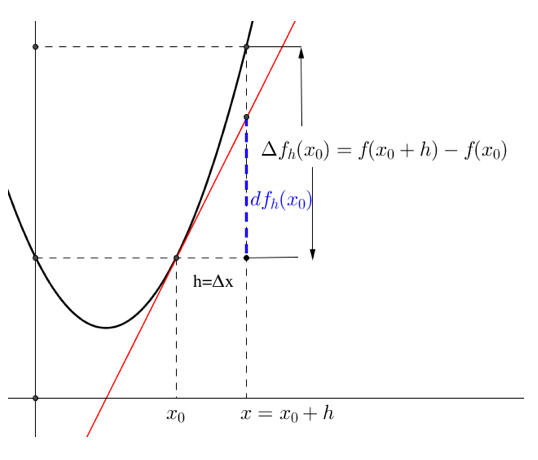
\includegraphics[width=0.40\textwidth]{imagenes/imagenes04/T04IM13.png}
			\caption {La Diferencial.}
		\end{figure}
			
		\end{multicols}	
		
		
		Estamos aproximando el valor de una función en un punto de difícil cálculo, $f(x_0+h)$, por el valor de esa función en un punto cercano y fácil de calcular, $f(x_0)$, y un término lineal (polinomio de primer grado) en $h$, $f'(x_0)\cdot h$. Esta aproximación será mejor cuanto menor sea $h$ y es \textit{la primera aproximación de una función}: en vez de considerar el crecimiento de la función $f(x_0+h)$, tomamos lo que crece su recta tangente $f(x_0)+f'(x_0)\cdot h$. Tomando derivadas de orden superior se encuentran polinomios de mayor grado que proporcionan mejores aproximaciones, son los desarrollos en serie de Taylor que veremos en futuros capítulos..
		
	
	
		En la práctica se usa:  $h=\Delta x= dx$ que se llama \textit{diferencial de x} (una cantidad muy pequeña -infinitesimal- en notación de Leibniz). Así: $df(x)=f'(x)\cdot dx = \dfrac {\dd f(x)}{\dd x}\dd x$
		
		\begin{ejem} Calcula un valor aproximado de $\sqrt{15.8}$
		
		Consideremos la función $f(x)=\sqrt{x}$, que es fácil calcular en el punto $x_0=16$, pero que es difícil calcular en el punto $x_0+h=15.8\to h=-0.2$. Como $f(x_0)=f(16)=\sqrt{16}=4; $ y $\; f'(x)=\dfrac {1}{2\sqrt{x}}\to f'(x_0)=f'(16)=\dfrac {1}{2\sqrt{16}}=\dfrac 1 8$, tendremos:
		
		$f(x_0+h)\simeq f(x_0)+f'(x_0)\cdot h$ 
		
		$f(16-0.2)=f(15.8)=\sqrt{15.8}\simeq f(16)+f'(16)\cdot (-0.2)=4+\dfrac 1 8 (-0.2)=4-0.025=3.975 \qquad $  \textcolor{gris}{El verdadero valor es $\sqrt{15.8}=3,974921382870358$}
			
		\end{ejem}
		
		\begin{ejem} Calcula $\dd (\ln \sqrt{1-\sin x})$
		
		$\dd y = f'(x) \dd x \to \dd (\ln \sqrt{1-\sin x})= \dfrac {1}{\sqrt{1-\sin x}} \dfrac {1}{2\sqrt{1-\sin x}}(-\cos x)\; \dd x=\dfrac {\cos x}{2(\sin x - 1)} \dd x$	
			
		
					
		\end{ejem}
		
		\begin{ejem} Las dimensiones de un cilindro son $5 \; dm$ de altura y $2 \; dm$ de radio. Calcula un valor aproximado de la variación que experimenta el volumen del cilindro si, manteniéndose constante la altura, el radio aumente en un $3 \%$
		
		El volumen del cilindro viene dado por la expresión $V=\pi r^2 \; h$. Si suponemos que la $h$ se mantiene constante, tenemos $V(r)=\pi r^2 \; h$. Al pasar el radio del valor $r=2\; dm$ al valor $r+\dd r=2+ 0.03\cdot 2=2.06 \; dm$, el volumen experimentará un cambio $\Delta V=V(r+\dd r)-V(r)$, pero estamos buscando una aproximación con la diferencial:
		
		$\Delta V \approx \dd  V =  \pi \; 2 r \; \dd r\; h= 2 \pi h r \dd r = 2 \pi \; 5 \cdot 2 \cdot 0.06 \approx 3.77 \; dm^3$ 
		\end{ejem}
		
			\section{Ejercicios de derivadas}
	\subsection{Ejercicios resueltos de derivadas}
	
	\begin{ejre} Utilizando la definición de derivada, calcula $f'(2)$ para los siguientes casos:
	
	$a) \quad f(x)=\dfrac {x-1}{x+1}; \qquad b) \quad f(x)=\sqrt{x+2}$
	\end{ejre}
	
	\begin{proofw}\renewcommand{\qedsymbol}{$\diamond$}
	
	$a) \quad f'(2)=\underset{x\to 2}{lim}\;{\dfrac {f(x)-f(2)}{x-2}}= \underset{x\to 2}{lim}\; {\dfrac {\dfrac {x-1}{x+1}-\dfrac 1 3}{x-2}}=\underset{x\to 2}{lim}\; {\dfrac {3(x-1)-(x+1)}{3(x+1)(x-2)}}=\underset{x\to 2}{lim}\; {\dfrac {2\cancel{(x-2)}}{3(x+1)\cancel{(x-2)}}}=\dfrac 2 9$
	
	$b) \quad f'(2)=\underset{h\to 0}{lim}\;{\dfrac {f(2+h)-f(2)}{h}}=\underset{h\to 0}{lim}\;{\dfrac {\sqrt{h+4}-2}{h}}=[0/0;\mbox{ ind }]= \underset{h\to 0}{lim}\;{\dfrac {\sqrt{h+4}-2}{h}}\cdot \dfrac {\sqrt{h+4}+2}{\sqrt{h+4}+2}=\underset{h\to 0}{lim}\;{\dfrac {\cancel{h}}{\cancel{h}\cdot(\sqrt{h+4}+2) }}=\dfrac 1 4$
	
	\end{proofw}
	
	\begin{ejre} Determina la diferencial para cada una de las siguientes funciones: $f(x)=x^4-2x^2+1;\quad g(x)=e^{2x^2+1}$	
	\end{ejre}
	
	\begin{proofw}\renewcommand{\qedsymbol}{$\diamond$}
	
	$\dd f= (4x^3-4x)\; \dd x \qquad \dd g= 4x\; e^{2x^2+1}\; \dd x$
	\end{proofw}
	
	\begin{ejre} Calcula un valor aproximado de las expresiones: $\quad \dfrac 1 {4.001}; \quad \dfrac {1}{2,01^3}$	
	\end{ejre}
	
	\begin{proofw}\renewcommand{\qedsymbol}{$\diamond$}
	
	$\dfrac 1 {4.001} \to f(x)=\dfrac 1 x;\quad x_0+h=4.001;\quad h=0.001; \quad x_0=4; \quad f'(x)=-\dfrac 1 {x^2}$
	
	$f(x_0+h) \approx f(x_0)+f'(x_0) \cdot h \Rightarrow \dfrac 1 {4.001} \approx 0.25 + (-0.0625)\cdot 0.01 \approx 0.24994$
	
	$\quad$
	
	$\dfrac {1}{2,01^3} \to f(x)=\dfrac 1 {x^3};\quad x_0+h=2.01;\quad h=0.01; \quad x_0=2; \quad f'(x)=-\dfrac 3 {x^4}$
	
	$f(x_0+h) \approx f(x_0)+f'(x_0) \cdot h \Rightarrow \dfrac 1 {2,01^3} \approx 0.125 + (-0.1875)\cdot 0.01 \approx 0.12313$
	\end{proofw}

	\begin{ejre} 	Comprueba que la siguiente función es continua y derivable. Calcula $f'(0);\; f'(1);\; f'(3)$. Calcula $f'(x)$ y comprueba si hay algún punto en que $f'(x)=5$
	
			$f(x)=
		\begin{cases}
		3x-1 & \mbox{ si } x< 1 \\
		x^2+x & \mbox{ si } x\ge 1  
		\end{cases} ;$
	\end{ejre}
	
	\begin{proofw}\renewcommand{\qedsymbol}{$\diamond$}
	
	Continuidad de $f(x)$ en $x=1$, en el resto siempre continua (polinomios):
	
	$1) \quad \exists f(1)=1^2+1=2$
	
	$2) \quad \exists \underset{x\to 1^-}{lim}\;{3x-1}=2=\underset{x\to 1^+}{lim}\;{x^2+x}=\underset{x\to 1}{lim}\;{f(x)}$
	
	$3) \quad $Coinciden, luego $f(x)$ es continua en $x=1$. Para ver si es derivable estudiaremos si coinciden sus derivadas laterales a partir de $f'(x)$.
	
	Calculemos, ahora, $f'(x)$ derivando solo en los intervalos abiertos:
	
	$f'(x)=
		\begin{cases}
		3 & \mbox{ si } x< 1 \\
		2x+1 & \mbox{ si } x >1  
		\end{cases} ; \qquad \mbox{?`} \exists f'(1)?$
		
		$f'_-(1)=\underset{x\to 1^-}{lim}\;{f'(x)}=\underset{x\to 1^-}{lim}\;{3}=3$
		
		$f'_+(1)=\underset{x\to 1^+}{lim}\;{f'(x)}=\underset{x\to 1^+}{lim}\;{2x+1}=3$
		
		Como $f'_-(1)=3=f'_+(1) \Rightarrow \exists f'(1)=3$. Muchos autores reescriben la función derivada incluyendo este último resultado, $f'(1)=3$, por ejemplo así:
		
			$f'(x)=
		\begin{cases}
		3 & \mbox{ si } x\le 1 \\
		2x+1 & \mbox{ si } x >1  
		\end{cases} $
		
		Contestemos ahora a las restantes preguntas $f'(0)= 3;\quad f'(1)=3;\quad  f'(3)=7$
		
		Probemos, por último, si $\exists x \; / \;  f'(x)=5$
		
		$\mbox{si }x\le 1 \to f'(x)=3 \neq 5$. Para $x\le 1$ la ecuación propuesta $f'(x)=5$ no tiene solución.
		
		$\mbox{si }x> 1 \to f'(x)=2x+1 =5 \leftrightarrow x=2 \in ]1,+\infty[$. Para $x> 1$ la ecuación propuesta $f'(x)=5$ sí tiene solución, $x=2$.
		
	
	\end{proofw}
	
	\begin{ejre} 	Calcula los valores de $m$ y $n$ para que $f$ sea derivable en todo $\mathbb R$ 
	
		$f(x)=
		\begin{cases}
		x^2-5x+m & \mbox{ si } x\le 1 \\
		-x^2+nx & \mbox{ si } x >1  
		\end{cases} $
		
		?`En qué puntos es $f'(x)=0$?
	\end{ejre}
	
	\begin{proof}[]
	\renewcommand{\qedsymbol}{$\diamond$}
	
	Por ser una función a trozos, ambos polinómicos, $f(x)$ es continua en todo $\mathbb R$ excepto, tal vez, en el nexo $x=1$ donde estudiamos la continuidad con el método de los tres pasos:
	
	$1) \quad \exists f(1)=1^2-5+m=-4+m$
	
	$2) \quad \exists \underset{x\to 1^-}{lim}\;{x^2-5x+m}=-4+m$
	$ \exists \underset{x\to 1^+}{lim}\;{-x^2+nx}=-1+n$
	Para que $\exists \underset{x\to 1}{lim}\;{f(x)}$, los límites laterales han de coincidir, por lo que: $-4+m=-1+n \to m-n=3 \quad (1*)$
	
	$3) \quad$ Coinciden siempre que se cumpla la condición $(1*)$ y $f(x)$ será continua en $x=1$ y, probablemente derivable.
	
	Estudiemos fa función derivada:
	
	$f'(x)=
		\begin{cases}
		2x-5 & \mbox{ si } x< 1 \\
		-2x+n & \mbox{ si } x >1  
		\end{cases} ; \qquad \mbox{?`} \exists f'(1)?$
		
	$f'_-(1)=2-5=-3; f'_+(1)=-2+n \Rightarrow $ Para que $\exists f'(1)$, las derivadas laterales debe coincidir, por lo que exigimos que $-3=-2+n \to n=-1 \quad (2*)$
	
	De las condiciones exigidas $(1*)$ y $(2*)$ tenemos un sistema de dos ecuaciones con dos incógnitas cuya solución es:
	
	$\begin{cases}
		m-n=3 \\
		n=-1
	\end{cases}  \qquad \Rightarrow \qquad m=2 \; \wedge \; n=-1$
	
	Recopilando, escribimos ahora $f'(x)$ como queda y estudiaremos si $f'(x)=0$ tiene solución.
	
	$f'(x)=
		\begin{cases}
		2x-5 & \mbox{ si } x\le 1 \\
		-2x-1 & \mbox{ si } x >1  
		\end{cases}$
	
	Para $x\le 1 :\; f'(x)=2x-5=0 \mbox{ si } x=\dfrac 5 2 = 2.5 \notin ]-\infty,1[ $. No hay solución.
	
	Para $x> 1 : \; f'(x)=-2x-1=0 \mbox{ si } x=-\dfrac 1 2 = -0.5 \notin ]1,+\infty[ $. No hay solución.
	
	Luego, $\nexists x \; / \; f'(x)=0$. Esta función no tiene puntos de derivada nula.
	\end{proof}
	
\begin{ejre} Calcula $f'$ y $f''$ para la función:
	
	$f(x)=x\cdot |x|=
	\begin{cases}
		-x^2 & \mbox { si } x<0 \\
		x^2  & \mbox { si } x\ge 0
	\end{cases}$	
	\end{ejre}
	
	\begin{proofw}\renewcommand{\qedsymbol}{$\diamond$}
	La función es continua en todo $\mathbb R$ excepto, tal vez, en $x=0$ por ser nexo. Pero, abreviando: $f-(0)=0=f_+(0)=f(0)$, continua en $x=0$, continua en todo $\mathbb R$.
	
	$f'(x)=
		\begin{cases}
		-2x & \mbox{ si } x< 0 \\
		2x & \mbox{ si } x >0  
		\end{cases} ; \qquad  \exists f'(0)=f'_-(0)=f'_+(0)=0$
		
		La función derivada $f'$ también es continua en todo $\mathbb R$:
		
	$f'(x)=
		\begin{cases}
		-2x & \mbox{ si } x< 0 \\
		2x & \mbox{ si } x \ge0  
		\end{cases}$	
		
		Calculemos la derivada segunda:
		
	$f''(x)=
		\begin{cases}
		-2 & \mbox{ si } x< 0 \\
		2 & \mbox{ si } x >0  
		\end{cases} ; \qquad   f''_-(0)=-2 \neq f''_+(0)=2 \to \nexists f''(0)$	
		
		Es decir:
		
		$f''(x)=
		\begin{cases}
		-2 & \mbox{ si } x< 0 \\
		2 & \mbox{ si } x >0  
		\end{cases}$
		
		Conclusión: $f'$ es continua en todo $\mathbb R$, pero $f''$ solo es continua en $\mathbb R \sim \{0\}$
	
	\end{proofw}
	
	\begin{ejre} 	Estudia la derivabilidad de la función 
	$f(x)=\dfrac 1 {1+|x|}$
	\end{ejre}
	
	\begin{proofw}\renewcommand{\qedsymbol}{$\diamond$}
	
	$f(x)=\dfrac 1 {1+|x|}=
	\begin{cases}
		\dfrac 1 {1-x} & \mbox{ si } x<0 \\
		\dfrac 1 {1+x} & \mbox{ si } x\ge0
	\end{cases}$
	
	Función continua en todo $\mathbb R$ por que sus denominadores no se anulan nunca ($1-x\neq 0, \; x<1$ y $1+x\neq 0, \; x\ge1$). Además, $f_-(0)=1=f_+(0)=f(0)$, la función es continua en el $0$.
	
	Calculemos la función derivada:
	
		$f'(x)=
		\begin{cases}
		\dfrac {1}{(1-x)^2} & \mbox{ si } x< 0 \\
		\dfrac {-1}{(1+x)^2}  & \mbox{ si } x >0  
		\end{cases} ; \qquad   f'_-(0)=1 \neq f'_+(0)=-1 \to \nexists f'(0)$	
		
	La función es derivable en todo $\mathbb R \sim \{0\}$; en $x=0$ hay un P.A.
	
	\end{proofw}
	
	\begin{ejre} $f(x)=\begin{cases}
	\dfrac {1}{1+e^{\dfrac 1 x}} & \mbox{ si } x \neq 0 \\
	0 & \mbox{ si } x=0
	\end{cases}$. Estudia la continuidad de $f(x)$ y calcula $f'(1)$.
		
	\end{ejre}
	
	\begin{proofw}\renewcommand{\qedsymbol}{$\diamond$}
	
	Continuidad de $f$ en $x=0$, resto continua.
	
	$1) \quad f(0)=0$
	
	$2) \quad \nexists \underset{x\to 0}{lim}\;{f(x)}$ porque los límites laterales son finitos pero distintos.
	
	$\underset{x\to 0^-}{lim}\;{\dfrac {1}{1+e^{\dfrac 1 x}}}=\dfrac {1}{1+e^{\dfrac 1 {-0}}}=\dfrac {1}{1+e^{-\infty}}=\dfrac {1}{1+0}=1$
	
	$\underset{x\to 0^+}{lim}\;{\dfrac {1}{1+e^{\dfrac 1 x}}}=\dfrac {1}{1+e^{\dfrac 1 {+0}}}=\dfrac {1}{1+e^{+\infty}}=\dfrac {1}{1+\infty}=\dfrac 1 \infty=0$
	
	$3) \quad $ No coinciden. $f$ es discontinua de salto en $x=0$ ($\to \nexists f'(0)$)
		
	$f'(x)= -\dfrac {1}{\left( 1+e^{\dfrac 1 x} \right)^2} e^{\dfrac 1 x} \left( -\dfrac 1 {x^2}\right)=\dfrac {e^{\dfrac 1 {x}}}{x^2\; \left( 1+e^{\dfrac 1 x} \right)^2} \to f'(1)=\dfrac e {(1+e)^2}$
		
	\end{proofw}
		
	\begin{ejre} El radio de un círculo crece a una velocidad de  $2\; m/s$	. Encuentra la velocidad de crecimiento del área del círculo cuando el radio es de $5\; m$. Haz lo mismo si se trata de una esfera, calcula la velocidad con que crecería el volumen en esas condiciones.
	\end{ejre}
	
	\begin{proofw}\renewcommand{\qedsymbol}{$\diamond$}
	
	\hspace{5mm} $r(t)=2t\; m/s;\; r(m);\; t(s)$
	
	$S(t)=\pi \; r^2(t)=\pi\; (2t)^2= 4\pi t^2$
	
	La velocidad de crecimiento del área la da su derivada:
	
	$S'(t)=8\pi\; t \qquad \mbox{ si } r=5=2t \to t=5/2\; s \Rightarrow S'(5/2)=8\pi \dfrac 5 2 = 20 \pi \; cm^2/s $
	
	Para el volumen de la esfera: $V=\frac 4 3 \pi \; r^3$ y la velocidad de crecimiento:
	
	$V'(t)=\dfrac 4 3 \pi 3r^2=4\pi r^2 \Rightarrow V'(5/2)=4\pi \dfrac 5 2=10\pi \; cm^3/s$
	
	\end{proofw}
	
	
	\begin{ejre} 	La altura de un triángulo equilátero aumenta a una velocidad de $3\; cm/s$. Calcula la velocidad a la que aumentará el área cuando la altura sea de $5\; cm$.
	\end{ejre}
	
	\begin{proofw}\renewcommand{\qedsymbol}{$\diamond$}
	 
	\begin{multicols}{2}
	
	\begin{figure}[H]
		\centering
		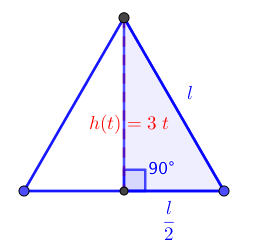
\includegraphics[width=0.3\textwidth]{imagenes/imagenes04/T04IM14.png}
	\end{figure}
		$h(t)=3t; \; t(s);\; h(cm)$
		
		Pitágoras: $l^2= \left(\dfrac l 2 \right)^2+ h^2$
		
	
		$ l=\dfrac {2 \sqrt{3}}{3}\; h \to l(t)=\dfrac {2 \sqrt{3}}{3} \; 3t =2 \sqrt{3} \; t$
		
		
		
		$S(t)=\dfrac 1 2 l(t) \cdot h(t)= \dfrac 1{ \cancel{2}} \cancel{2} \sqrt{3} t \cdot 3t=3 \sqrt{3} t^2$
		\end{multicols}
		La velocidad de crecimiento del área es su derivada:
		


	$S'(t)= \dv {S(t)}{t}=3\sqrt{3}\cdot 2t= 6\sqrt{3}t$. Cuando $h=5=3t \to t=5/3\; s \Rightarrow S'(5/3)=6\sqrt{3}\cdot \dfrac 5 3=10\sqrt{3}\; cm^2/s$
	
	\end{proofw}
	
	
	\begin{ejre} Un depósito esférico elástico, de $10\; cm$ de radio, lleno de He, se vacía a razón de $-1\; l/min$. Calcula la velocidad de disminución de la superficie del depósito cuando el radio se reduce a la mitad.
		
	\end{ejre}
	
	\begin{proofw}\renewcommand{\qedsymbol}{$\diamond$}
		
	$r_0=10\; cm = 1 \; dm$. Trabajaremos las distancias en $dm$, áreas en $dm^2$ y, así, volúmenes en $dm^3=l$.
	
	$V_0=\frac 4 3 \pi r_0^3=\frac {4\pi}{3}\; l \to V(t)=\frac {4\pi}{3}-t; \quad V(l); \; t(min)$
	
	$\frac {4\pi}{3}-t=\frac {4\pi}{3}r^3(t) \to r(t)=\sqrt[3]{1-\frac {3}{4\pi}t}$
	
	Cuando el radio se reduce a la mitad: $0.5=\sqrt[3]{1-\frac {3}{4\pi}t} \to \frac 1 8 = 1-\frac {3}{4\pi}t \to t=\frac {7\pi}{6} min$
	
	$S(t)=4\pi r^2(t)=4\pi \left( 1 - \frac {3}{4\pi} t \right)^{2/3}$
	
	$S'(t)=4\pi \frac 2 3 \left( 1 - \frac {3}{4\pi} t \right)^{-1/3} \left( \frac {-3}{4\pi} \right)= -2 \left( 1 - \frac {3}{4\pi} t \right)^{-1/3}$
	
	$S'(\frac {7\pi}{6})=-2 \left(1- \frac {3}{4\pi} \frac {7\pi}{6} \right)^{\frac {-1}{3}}= -2 \left( 1-\frac 7 8 \right)^{\frac {-1}{3}}=\frac {-2}{\sqrt[3]{1/8}}=-4 \; dm^2/min$
		
	\end{proofw}
	
	
	\begin{ejre} Vaciado de un tanque.
	
	\begin{multicols}{2}
	
	\begin{figure}[H]
	\centering
	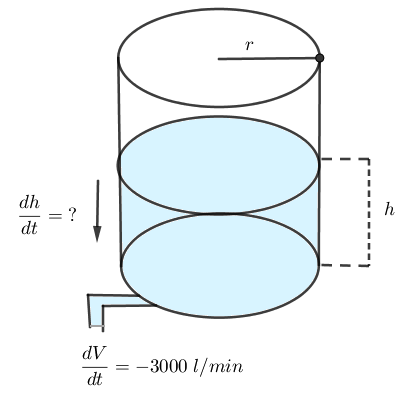
\includegraphics[width=0.3\textwidth]{imagenes/imagenes04/cilindro.png}
	\end{figure}
	
	$\quad$
	
	?`Qué tan rápido baja el nivel de líquido en un tanque cilíndrico vertical, si lo drenamos a una razón de $3000 \; l/min$?
		
	\end{multicols}

	\end{ejre}
	
	\begin{proofw}\renewcommand{\qedsymbol}{$\diamond$}
		
	Vamos a medir $r(m)$ y $h(m)$ con lo cual, el volumen del cilindro será $V=\pi r^2\; h \; (m^3) = 1000 \pi r^2\; h (l)$, ya que $1 \; m^3 = 1000 \; l$.
	
	Vamos a resolver el problema usando la notación de Leibniz para la derivada.
	
	A medida que pasa el tiempo $t$, tendremos que tanto el volumen como la altura del líquido en el cilindro serán función de $t: \quad V(t); \; h(t)$.
	
	Derivemos la expresión 	$V(t)=1000 \pi r^2 \; h(t)$ respecto del tiempo $t$:
	
	$\dv {V}{t}= 1000\pi r^2\; \dv {h}{t}$, $\quad r$ es constante. Como $\dv {V}{t}=-3000$, despejando $\dv {h}{t}$ obtenemos:
	
	$\dv {h}{t}= - \frac {3000}{1000 \pi r^2}=\frac {-3}{\pi r^2}\; m/min$.
	
	La velocidad con que baja el líquido en el tanque es inversamente proporcional al cuadrado del radio del mismo, si $r$ es grande, el líquido bajará a poca velocidad, pero si $r$ es pequeño, el líquido bajará a mayor velocidad.
	
	\textcolor{gris}{El mismo problema resuelto con notación de Lagrange sería:}
	
	\textcolor{gris}{$V(t)=1000\pi r^2 h(t); \quad V`(t)=-3000\; l/min \to V'=1000 \pi r^2 h'=-3000$}
	
	\textcolor{gris}{$ \to h'(t)=-\frac 3 {\pi r^2}\; m/min$}
		
	\end{proofw}
	
	\begin{ejre} El globo ascendente.
	
	
	
	\begin{multicols}{2}
	
	\begin{figure}[H]
	\centering
	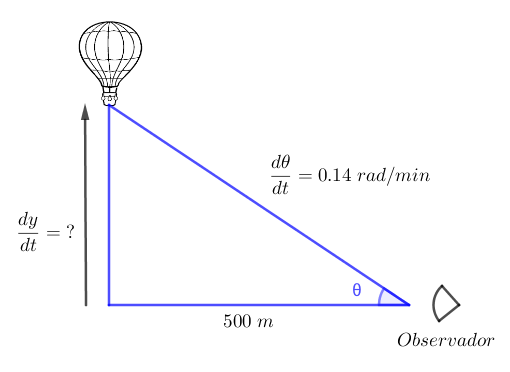
\includegraphics[width=0.4\textwidth]{imagenes/imagenes04/globo.png}
	\end{figure}
	Un globo aerostático que asciende en línea recta desde el nivel del suelo es rastreado por un observador que está a $500\; m$  del punto de elevación. El momento en el que el ángulo de elevación es de $\pi/4$, el ángulo crece a razón de $0.14\; rad/min$. ?`Qué tan rápido se está elevando el globo en ese momento? 		
	\end{multicols}

		
	\end{ejre} 
	
	
	\begin{proofw}\renewcommand{\qedsymbol}{$\diamond$} 
	
También usaremos la notación de Leibniz en la resolución de este problema.
	
	Tenemos: $t(min); \quad \theta (t); \quad y(t)$. Además, $\dv {\theta}{t}=0.14 \; rad/min \mbox{  cuando  } \theta=\pi/4$.
	
	Queremos encontrar $\dv {y}{t}$ en el instante en que $\theta=\pi/4$.
	
	De la figura observamos que: $\frac y {500}=\tan \theta \to y=500 \tan \theta$
	
	Usando la regla de la cadena y derivando respecto a $t$, tenemos que:
	
	$\dv {y}{t}=\frac {500}{\cos^2 \theta} \dv {\theta}{t} \quad to \quad $. En $\theta=\pi/4$ y $\dv {\theta}{t}=0.14 \quad $
	
	$\to \dv {y}{t}=140 \; m/min \qquad \textcolor{gris}{(\cos(\pi/4)=\sqrt{2}/
	2)}$ 
		
	\end{proofw}


	\subsection{Ejercicios propuestos de derivadas}
	
	\emph{Los problemas de encontrar rectas tangentes y normales a una función en un punto los dejaremos para el siguiente capítulo de `Aplicaciones de las derivadas'.}

	\begin{enumerate}
		\item Deriva las siguientes funciones:
		
		
		$a) \quad y=\dfrac {\sin x}{1+\cos x} \Rightarrow \textcolor{gris}{y'=\dfrac {1}{1+\cos x}}$
		
		$b) \quad y=\cos (\sin^2 5x)   \Rightarrow \textcolor{gris}{ y'= -10 \sin 5x\; \cos 5x\; \sin(\sin^2 5x) }$	
		
		$c) \quad y= \tan(5x-7)  \Rightarrow \textcolor{gris}{ y'=\dfrac {5}{\cos^2 (5x-7)} }$
		
		$d) \quad y=2\sqrt{\cos 3x}   \Rightarrow \textcolor{gris}{ y'= -\dfrac{6\sin 3x}{\sqrt{\cos 3x}}}$
		
		$e) \quad y=\ln \sqrt{\dfrac {1 + \sin x}{1-\sin x}}   \Rightarrow \textcolor{gris}{ y'= \dfrac 1 {\cos x}}$
		
		$f) \quad y= \ln(\sin^2 x)  \Rightarrow \textcolor{gris}{ y'= \dfrac 2 {\tan x}}$
		
		$g) \quad y= \ln(\cos x)  \Rightarrow \textcolor{gris}{ y'= - \tan x }$
		
		$h) \quad y=x^{\sin x}   \Rightarrow \textcolor{gris}{ y'=\left( \cos x \; \ln x + \dfrac {\sin x}{x}  \right) }\cdot x^{\sin x}$
		
		$i) \quad y= \sqrt[\tan x]{x}  \Rightarrow \textcolor{gris}{ y'=\dfrac {\sin x \; \cos x - \ln x}{x\;  \cos^2x\; \sin^2 x} }\cdot \sqrt[\tan x]{x}$
		
		$j) \quad y= e^{\ln (\atan \sqrt
		x)}  \Rightarrow \textcolor{gris}{ y'= \dfrac 1 {2(1+x)\sqrt{x}} }$
		
		$k) \quad y=\dfrac {1}{\sqrt{5}} \arcsin \left( \dfrac {3\cos x + 2}{3+2\cos x} \right)   \Rightarrow \textcolor{gris}{ y'= -\dfrac {1}{3+2\cos x}}$
		
		$l) \quad y=\arccos \left(\dfrac {1-x^2}{1+x^2} \right)   \Rightarrow \textcolor{gris}{ y'= \dfrac {2}{1+x^2}}$
		
		$m) \quad y= \arctan \left(\dfrac {3 \sin x}{4+5\cos x} \right)  \Rightarrow \textcolor{gris}{ y'= \dfrac {3}{5+4\cos x} }$
		
		$n) \quad y= \sqrt { 1+\sqrt{x} }  \Rightarrow \textcolor{gris}{ y'=\dfrac {1}{4 \sqrt{x} \sqrt{\sqrt{x}+1}} } $
		
		$o) \quad y= \ln \sqrt{\dfrac {1+x}{1-x}}  \Rightarrow \textcolor{gris}{ y'= \dfrac {1}{1-x^2}}$
		
		$p) \quad y= 7^{x^2+2x}  \Rightarrow \textcolor{gris}{ y'= 2(x+1)\; \ln 7 \; 7^{x^2+2x} }$

		$q) \quad y= \dfrac {e^x-1}{e^x+1}  \Rightarrow \textcolor{gris}{ y'=\dfrac {2e^x}{(e^x+1)^2} }$
		
		$r) \quad y= x^2 \sin x + 2x \cos x -2 \sin x  \Rightarrow \textcolor{gris}{ y'= x^2\cos x}$
		
		$s) \quad y= \sin (2x) +\sin^2 x + \sin^2(2x)  \Rightarrow \textcolor{gris}{ y'= 2\cos(2x)+ 2 \sin x \; \cos x+ 4 \sin(2x) \; \cos (2x)}$
		
		$t) \quad y= \ln \sqrt{x^2+x+1}-\frac {1}{\sqrt{3}}\arctan \dfrac {2x+1}{\sqrt{3}}  \Rightarrow \textcolor{gris}{ y'= \dfrac {x}{x^2+x+1}}$

		$u) \quad y=\dfrac {\cos 2x + \sin 2x}{\cos 2x - \sin 2x}   \Rightarrow \textcolor{gris}{ y'= \dfrac {4}{(\cos 2x - \sin 2x)^2} }$
		
		$v) \quad y= \arcsin \left(\dfrac {1}{\ln x} \right)  \Rightarrow \textcolor{gris}{ y'=\dfrac {-1}{x\; \ln x \; \sqrt{(\ln x)^2-1}} }$
		
		$w) \quad 4x^2+y^2+4x-12y-6=0   \Rightarrow \textcolor{gris}{ y'= \dfrac {4x+2}{y+6}}$
		
		$x) \quad xy=e^x+y   \Rightarrow \textcolor{gris}{ y'= \dfrac {e^x-y}{x-1}}$
		
		$y) \quad \sqrt{xy}=\ln y   \Rightarrow \textcolor{gris}{ y'= \dfrac {y^2}{2\sqrt{xy}-xy}}$
		
		$z) \quad \sin(3x^2y^5)+e^{x^2+y^2}=2xy^3   \Rightarrow \textcolor{gris}{ y'= \dfrac {2y^3-6xy^5\cos(3x^2y^5)-2xe^{x^2+y^2}}{15x^2y^4\cos(3x^2y^5)+2ye^{x^2+y^2}-6xy^2} }$
		
		\item Aplica la definición de derivada para calcular en cada caso: 
		
		$a)\quad f(x)=x+\dfrac 1 x;\qquad b) \quad g(x)=\sqrt{x^2+1}$
		
		\rightline{\textcolor{gris}{Solución: $a)\quad f(x)=1 - \dfrac 1 {x^2}; \qquad b)\quad g(x)=\dfrac {x}{\sqrt{x^2+1}}$}}
		
		\item Determina $\dd f$ para cada una de las funciones siguientes:
		
		$a)\quad f(x)=\ln \dfrac {4}{x^2} \qquad b)\quad f(x)=\sqrt[3]{x^2+2}$
		
		\rightline{\textcolor{gris}{Solución: $a)\quad \dd f= -\dfrac 2 x \; \dd x; \qquad b)\quad \dd f= \dfrac {2x\; \sqrt[3]{x^2+2}}{3(x^2+2)} \; \dd x$ }}
		
		\item Usando la diferencial, calcula un valor aproximado de:
		
		$\sqrt{122}; \qquad \sqrt{1370}; \qquad \log_2 130; \qquad \sqrt[4]{260}; \qquad \sqrt[3]{103825}; \qquad 3^{4.001};\qquad  \log 10001$
		
		
		\rightline{\textcolor{gris}{Solución: $11.045;\quad 37.014;\quad 7.0225;\quad 4.3536;\quad 47.0003;\quad 81.089; \quad 4.000043$}}
		
		\item Estudia la continuidad y derivabilidad de las siguientes funciones:
	
	
	\begin{multicols}{2}
		
		
		$f(x)=
	\begin{cases}
		e^x & \mbox{ si } x\le 0 \\
		1 & \mbox{ si } 0<x<3 \\
		-x^2+3x+2 & \mbox{ si } x\ge 3 
	\end{cases} ;$
	
	$g(x)=
	\begin{cases}
		x^2+2x+1 & \mbox{ si } x< -1 \\
		2x+2 & \mbox{ si } -º \le x \le 2 \\
		-x^2+8x & \mbox{ si } x>2 
	\end{cases} ;$
		
	\end{multicols}
		
		\rightline{\textcolor{gris}{Solución:$f$ no continua en $x=3$, por tanto, no dvble. $f$ ctna. en $x=0$, pero no dvble., PA }}
		\rightline{\textcolor{gris}{$g$ es continua en $x=-1$, pero no dvble., PA. $g$ es no continua en $x=2$, por tanto, no dvble.}}
		
		\item Calcula las derivadas enésimas de las funciones:
		
		$a)\quad f(x)=e^{ax}; \qquad b) \quad g(x)=\ln (1+x)$
		
		
		\rightline{\textcolor{gris}{Solución: $a)\quad f^{n)}(x)= a^n\; e^{ax}\; ; \qquad g^{n)}(x)=\dfrac {(-1)^n \cdot (n-1)!}{x^{n+1}}$ }}
		
		
		\item Dada $f(x)=e^x \cos x$, demuestra que $f''(x)-2f'(x)+2f(x)=0$
		
		\rightline{\textcolor{gris}{Solución: sí se cumple.}}
		
		\item Calcula $a$ y $b$ para que las siguientes funciones sean derivables en todo $\mathbb R:$
	\begin{multicols}{2}
		
		$f(x)=
	\begin{cases}
		ax^2+3x & \mbox{ si } x\le 2 \\
		x^2-bx-4 & \mbox{ si } x>2 
	\end{cases} ;$
	
	$g(x)=
	\begin{cases}
		x^3-x & \mbox{ si } x\le  0 \\
		ax+b & \mbox{ si } x>0  
	\end{cases} $
	
	\end{multicols}

		
		\rightline{\textcolor{gris}{Solución: Para $f(x): \quad a=2; \; b=-7; \qquad $ Para $g(x): \quad a=-1; \; b=0$ }}
		
		\item $f:[0,5]\to \mathbb R:\; f(x)=\begin{cases}
		ax+bx^2 & \mbox{ si } 0\le x < 2 \\
		c+\sqrt{x-1}  & \mbox{ si } 2 \le x \le 5	
		\end{cases}$. Derivable en $]0,5[$ y con $f(0)=f(5)$. Determina $a$, $b$ y $c$
		
		\rightline{\textcolor{gris}{Solución: $a=-3/2; \; b=1/2; \; c=-2$}}
		
		
	\item Determina $a$ y $b$ para que sea continua y derivable la función:
	
	$f(x)=\begin{cases}
		\dfrac {1-x}{e^x} & \mbox{ si } x<0 \\
		x^2+ax+b & \mbox{ si } x\ge 0	
		\end{cases}$
		
	\rightline{\textcolor{gris}{Solución:$a=-2; \; b=1$ }}
		
	
	\item Determina el valor de $m$ para que la siguiente función sea continua. Calcula, si es posible, $f'(0)$.
	
	$f(x)=\begin{cases}
		m(x+1)e^{2x} & \mbox{ si } x\le 0 \\
		\dfrac {(x+1)\sin x}{x} & \mbox{ si } x > 0	
		\end{cases}$
		
	\rightline{\textcolor{gris}{Solución: $m=1; \quad \nexists f'(0):\; f'_-(0)=2 \neq f'_+(0)=+\infty$}}
		
		
		\item Estudia la continuidad y derivabilidad de $f(x)=|1-|x||$
		
		\rightline{\textcolor{gris}{Solución: Recordar como romper $f$ en trozos según el ejercicio \ref{ejre:rompe-trozos}}}
		\rightline{\textcolor{gris}{Continua en $\mathbb R$; derivable en $\mathbb R \sim \{-1,0,1\}$}}
		
		
		\item Estudia la continuidad y derivabilidad de $f(x)=x^2+2x-|x|$
		
		\rightline{\textcolor{gris}{Solución: Continua en $\mathbb R$; derivable en $\mathbb R \sim \{0\}$ }}
		
		
		\item Estudia la derivabilidad de las siguientes funciones:
		
		\begin{multicols}{2}
		\begin{enumerate}[a) ]
			\item $y=|x-2|$
			\item $y=|x^2+6x-8|$
			\item $y=x+|x-3|$ 
			\item $y=x^2+|x|$
		\end{enumerate}
			
		\end{multicols}

		
		\rightline{\textcolor{gris}{Solución: $a)\;$ derivable en todo $\mathbb R \sim \{2\}$; $\quad b)\;$ derivable en todo $\mathbb R \sim \{-4,-2\}$}}
		\rightline{\textcolor{gris}{ $c)\;$ derivable en todo $\mathbb R \sim \{3\}$; $\quad d)\;$ derivable en todo $\mathbb R \sim \{0\}$}}
		
		\item Calcula la continuidad y derivabilidad de la función: $f(x)=\dfrac {|x|}{x^2-1}$
		
		
		\rightline{\textcolor{gris}{Solución: $f(x)$ es continua en todo $\mathbb R \sim \{-1,1\}$ y derivable en todo $\mathbb R \sim \{-1,1\}$}}
		
		\item Determina el valor del parámetro $a$ para que la función $f$ sea derivable en todo su dominio de definición.
		
		$f(x)=
	\begin{cases}
	x\; \ln x & \mbox{ si } 0\le  x \le 1 \\
		a\; (1-e^{1-x}) & \mbox{ si } x>1  
	\end{cases} $
		
		\rightline{\textcolor{gris}{Solución: $a=1$}}
		
		\item Indica los puntos de derivada nula de las funciones:
		
		$a) \quad f(x)= \cos 2x - 2 \cos x; \qquad b) \quad g(x)=\sqrt{4x-x^2}$
		
		\rightline{\textcolor{gris}{Solución: $f(x)=0\to x=\dfrac \pi 3 + 2 k \pi;\; x= \dfrac {5\pi}{3}+2k\pi; \; \forall k\in \mathbb Z; \qquad g(x)=0 \to x=2$}}
		
		\item Determina el aumento de volumen experimentado por un ortoedro de $15\; dm$ de altura y cuya base es un cuadrado de $20\; dm$ de lado, sabiendo que éste aumenta en $1\; cm$ su longitud. Hazlo de forma exacta y de forma aproximada \emph{(por la diferencial)}.
		
		\rightline{\textcolor{gris}{Solución: $\Delta V=60.15\; dm^3;\quad \dd V \approx 60\; dm^3$}}
		
		\item. Encuentra la derivada de la siguiente función y comprueba que es una constante:
		
		$y= \arctan \sqrt{\dfrac {1-\cos x}{1+\cos x}};\; \mbox{ con } 0\le x < \pi$
		
		Ayuda: ten en cuenta la fórmula de la $\tan \left( \dfrac x 2 \right)$
		
		\rightline{\textcolor{gris}{Solución: $y=\dfrac x 2 \to y'=\dfrac 1 2$ }}
		
		
		\item Encuentra los valores de $a$ y $b$ para que $f(x)$ sea continua. Para esos valores, estudia la derivabilidad de $f(x)$
		
		$f(x)=
		\begin{cases}
		2x+a  & \mbox{ si } x < 1 \\
		ax+b  & \mbox{ si } -1 \le x < 0 \\
		3x^2+2  & \mbox{ si } x\ge 0 
		\end{cases} $
		
		\rightline{\textcolor{gris}{Solución: $f(x)$ será continua si $a=2$ y $b=2$. Es derivable en todo $\mathbb R \sim \{0\}$}}
		
		\item El radio de una esfera crece con una velocidad de $3\; cm/s$. Calcula la velocidad de crecimiento del volumen de la esfera cuando en radio mide $5 \; cm$.
		
		\rightline{\textcolor{gris}{Solución: Ayuda: $ r(t)=3t: \; r(m); t(s) \quad \mbox{ veloc. crecto. volumen: } 300\pi \; cm^3/s$ }}
		
		\item ?`Cuánto aumenta, aproximadamente, el lado de un cuadrado si el área pasa de $9\; m^2$ a $9.1 \; m^2$?
		
		\rightline{\textcolor{gris}{Solución: $0.017 \; m$}}
		
		\item Calcular una aproximación del volumen de chapa necesaria para construir una esfera hueca de $40\; cm$ de diámetro exterior y de espesor $0.2\; cm$.
		
		\rightline{\textcolor{gris}{Solución: $320\pi\; cm^3$}}
		
		\emph{`La derivada de una función mide la velocidad (instantánea) de cambio (crecimiento) de dicha función'}
		
		\item Se bombea gas a un globo esférico a razón de $6 \; m^3/min$. Si la presión se mantiene constante, ?`Cuál es la velocidad con que cambia el radio del globo cuando el diámetro es de $120\; cm$?
		
		\rightline{\textcolor{gris}{Solución: $1.326\; m/min$}}
		
		\item Una persona camina a una velocidad constante de $3\; m/s$ y se aleja horizontalmente, en línea recta, de una farola que se encuentra a $10\; m$ de altura. Sabiendo que la persona mide $1.70\; m$ de altura, calcula:
		
			$a)\quad $ La longitud de la sombra cuando la persona está a $5 \; m$ de la base de la farola.
			
			$b)\quad$ La velocidad de crecimiento de la sombra a los $t$ segundos de empezar a caminar.
			
		
		\rightline{\textcolor{gris}{Solución: $1.024\; m; \quad 0.614\; m/s$ }}
		
		\item Un móvil se mueve con velocidad constante de $2 \; m/s$ en el primer cuadrante, sobre la recta $x=1$, a partir del punto $M(1,0)$ situado a $1\; m$ del origen. Otener, razonadamente:
		
		$a) \quad$ Las coordenadas del punto $M(t)$ donde está situado el móvil al cabo de $t\; s$.
		
		$b) \quad$ La función $m(t)$ igual a la pendiente de la recta que para por el punto $O(0,0)$ i el punto $m(t)$
		
		$c) \quad$ La derivada de la función $m(t)$.
		
		\rightline{\textcolor{gris}{Solución: $M(t)=(1,2t);\quad m(t)=2t;\quad m'(t)=2$}}
		
		\item En un triángulo rectángulo, uno de los catetos mide $8\; cm$ y decrece a razón de $1\; cm/min$; el otro cateto mide $6\; cm$ y crece a razón de $2\; cm/min$. Calcula la velocidad a la que crece el área al cabo de 2 minutos.
		
		\rightline{\textcolor{gris}{Solución: $2\; cm^2/min$}}
		
		\item Un incendio crece en forma circular uniformemente. El radio del área quemada crece a velocidad constante de $1.8 m/min$. Calcula la velocidad de crecimiento del área del incendio cuando el radio llega a los $45\; m$.
		
		\rightline{\textcolor{gris}{Solución: $2035.75\; m^2/min$}}
	
	\vspace{4mm}
		
	\item Llenado de un tanque cónico.
		
	\begin{multicols}{2}
	\begin{figure}[H]
	\centering
	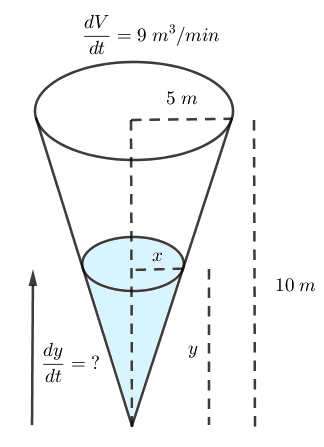
\includegraphics[width=0.3\textwidth]{imagenes/imagenes04/cono.png}
	\end{figure}
	
	En un tanque cónico, el agua entra a razón de $9\; m^3/min$. El tanque está colocado con el vértice hacia abajo y tiene una altura de $10\; m$ y el radio de su base es de $5\; m$. ?`Qué tan rápido sube el nivel del agua cuando la profundidad de la misma es xde $6\; m$?
	\end{multicols}
		
	\rightline{\textcolor{gris}{Solución: $0.32 \; m/min$}}
		
	\vspace{4mm}
	
	\item Vaciado de un depósito cónico.
	
	Un cono con el vértice invertido de $r=45\; m$ y $h=6\; m$ se está vaciando a razón de $50 \; m^3/m$. Calcular la velocidad a la que baja el nivel del líquido cuando el agua tiene $5\; m$ de profundidad y la velocidad con que cambia el radio en ese momento. 
	
	
	\rightline{\textcolor{gris}{Solución: $\eval {\dv {h}{t}}_{h=5}= -1.13\; cm/min; \quad \eval {\dv {r}{t}}_{h=5}=-8.5 \; cm/s$}}
	
	
 
		
	\item $\divideontimes$  Un globo y una bicicleta..
		
	\begin{multicols}{2}
	\begin{figure}[H]
	\centering
	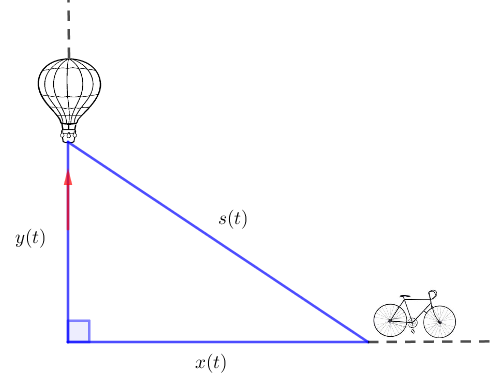
\includegraphics[width=0.4\textwidth]{imagenes/imagenes04/bici-globo.png}
	\end{figure}
	Un globo aeróstático se eleva dede una posición horizontal a una razón constante de $1\; m/s$. Justo cuando el globo está a $65 \; m$ sobre el suelo, una bicicleta que se mueve a una velocidad cosntante de $17\; m/s$ pasa por debajo de él. ?`Qué tan rápido aumenta la distancia $s(t)$ entre la bicicleta y el globo $3 \; s$ después.
	\end{multicols}
		
	\rightline{\textcolor{gris}{Solución: }}
		
		
		
		
		\item Considera las funciones:  $f(x)=\dfrac 1 2 \ln \dfrac {1+x}{1-x}$ y $g(x)=\ln \sqrt{\dfrac{1-x}{1+x}}$. Determina:
		
		$a) \quad$ Las derivadas de $f(x)$ y $g(x)$
		
		$b) \quad$ Los dominios de $f(x)$ y $g(x)$
		
		$c) \quad$ La expresión simplificada de $f(x)+g(x)$ y el recorrido de esta función.
		
		\rightline{\textcolor{gris}{Solución: $f'(x)=\dfrac 1 {1-x^2}=-g'(x); \quad D(f)=D(g)=]-1,1[$}}
		 \rightline{\textcolor{gris}{$f(x)+g(x)=0 \to Rec(f+g)=\{0\}$}}
		
		
		\item $\divideontimes$ Recordando la definición de funciones hiperbólicas dadas en la subsección \ref{subsec:func-hiperb}, comprueba que se cumplen las siguientes igualdades:
		
		\begin{enumerate}[a) ]
		\item $\cosh^2 x - \sinh^2 x=1$
		\item $\sinh(x+y)=\sinh x \cosh y + \cosh x \sinh y$
		\item $\cosh(x+y)=\cosh x \cosh y + \sinh x \sinh y$
		\item $\sinh' x= \cosh x$
		\item $\cosh'x=\sinh x$
		\item $\tanh'x=\dfrac {1}{\cosh^2 x}$
		
		\end{enumerate}
		
		
		
		
		
		\item $\divideontimes$ Encuentra solución para la ecuación: $f'(x)=f^{-1}(x)$
		
		\rightline{\textcolor{gris}{Ayuda: No hay más forma de intentar resolver el problema}}
		 \rightline{\textcolor{gris}{que probando por una función potencial $y=kx^n$}} 
		 \rotatebox{180}{\leftline{\textcolor{gris}{\scriptsize{más ayuda: $x^r=k \to r=0 \wedge k=1$} }}}
		 \rightline{\textcolor{gris}{Solución: $y=\dfrac {1}{\sqrt[\varphi+1]{\varphi}}x^{\varphi}$, con $\varphi$ el número de oro (también válida con $\varphi^{-1}$})}
		
	\end{enumerate}
	
	

	
	
	




	
